%
% The CCD Photometric Calibration Cookbook
%
% Copyright 1999  Starlink, CCLRC.
%
% A.C. Davenhall (Edinburgh), 22/4/99.
%

\documentclass[twoside,11pt]{article}

% ? Specify used packages
\usepackage{graphicx}        %  Use this one for final production.
% \usepackage[draft]{graphicx} %  Use this one for drafting.
% ? End of specify used packages

\pagestyle{myheadings}

% -----------------------------------------------------------------------------
% ? Document identification
% Fixed part
\newcommand{\stardoccategory}  {Starlink Cookbook}
\newcommand{\stardocinitials}  {SC}
\newcommand{\stardocsource}    {sc\stardocnumber}
\newcommand{\stardoccopyright} {Copyright \copyright\ 2001 Council for the
Central Laboratory of the Research Councils}

% Variable part - replace [xxx] as appropriate.
\newcommand{\stardocnumber}    {6.4}
\newcommand{\stardocauthors}   {J.~Palmer \& A.C.~Davenhall}
\newcommand{\stardocdate}      {31st August 2001}
\newcommand{\stardoctitle}     {The CCD Photometric Calibration Cookbook}
\newcommand{\stardocabstract}
{This cookbook presents simple recipes for the photometric calibration
of CCD frames.  Using these recipes you can calibrate the brightness
of objects measured in CCD frames into magnitudes in standard
photometric systems, such as the Johnson-Morgan {\it UBV}\, system.
The recipes use standard software available at all Starlink sites.

The topics covered include: selecting standard stars, measuring
instrumental magnitudes and calibrating instrumental magnitudes into a
standard system.  The recipes are appropriate for use with data acquired
with optical CCDs and filters, operated in standard ways, and describe the
usual calibration technique of observing standard stars.  The software
is robust and reliable, but the techniques are usually not suitable where
very high accuracy is required.

In addition to the recipes and scripts, sufficient background material
is presented to explain the procedures and techniques used.  The
treatment is deliberately practical rather than theoretical, in keeping
with the aim of providing advice on the actual calibration of observations.

\begin{latex}
\vspace{5mm}
\end{latex}

\begin{center}
{\bf Who Should Read this Cookbook?}
\end{center}

This cookbook is aimed firmly at people who are new to astronomical
photometry.  Typical readers might have a set of photometric observations
to reduce (perhaps observed by a colleague) or be planning a programme of
photometric observations, perhaps for the first time.  No prior knowledge
of astronomical photometry is assumed.

The cookbook is not aimed at experts in astronomical photometry.  Many
finer points are omitted for clarity and brevity.  Also, in order to
make the most accurate possible calibration of high-precision photometry,
it is usually necessary to use bespoke software tailored to the
observing programme and photometric system you are using.}
% ? End of document identification
% -----------------------------------------------------------------------------

% +
%  Name:
%     sc.tex
%
%  Purpose:
%     Template for Starlink Cookbook (SC) documents.
%     Refer to SUN/199
%
%  Authors:
%     AJC: A.J.Chipperfield (Starlink, RAL)
%     BLY: M.J.Bly (Starlink, RAL)
%
%  History:
%     16-JUN-1997 (BLY):
%        Original, based on SUN/SG templates.
%     {Add further history here}
%
% -

\newcommand{\stardocname}{\stardocinitials /\stardocnumber}
\markboth{\stardocname}{\stardocname}
\setlength{\textwidth}{160mm}
\setlength{\textheight}{230mm}
\setlength{\topmargin}{-2mm}
\setlength{\oddsidemargin}{0mm}
\setlength{\evensidemargin}{0mm}
\setlength{\parindent}{0mm}
\setlength{\parskip}{\medskipamount}
\setlength{\unitlength}{1mm}

% -----------------------------------------------------------------------------
%  Hypertext definitions.
%  ======================
%  These are used by the LaTeX2HTML translator in conjunction with star2html.

%  Comment.sty: version 2.0, 19 June 1992
%  Selectively in/exclude pieces of text.
%
%  Author
%    Victor Eijkhout                                      <eijkhout@cs.utk.edu>
%    Department of Computer Science
%    University Tennessee at Knoxville
%    104 Ayres Hall
%    Knoxville, TN 37996
%    USA

%  Do not remove the %begin{latexonly} and %end{latexonly} lines (used by 
%  star2html to signify raw TeX that latex2html cannot process).
%begin{latexonly}
\makeatletter
\def\makeinnocent#1{\catcode`#1=12 }
\def\csarg#1#2{\expandafter#1\csname#2\endcsname}

\def\ThrowAwayComment#1{\begingroup
    \def\CurrentComment{#1}%
    \let\do\makeinnocent \dospecials
    \makeinnocent\^^L% and whatever other special cases
    \endlinechar`\^^M \catcode`\^^M=12 \xComment}
{\catcode`\^^M=12 \endlinechar=-1 %
 \gdef\xComment#1^^M{\def\test{#1}
      \csarg\ifx{PlainEnd\CurrentComment Test}\test
          \let\html@next\endgroup
      \else \csarg\ifx{LaLaEnd\CurrentComment Test}\test
            \edef\html@next{\endgroup\noexpand\end{\CurrentComment}}
      \else \let\html@next\xComment
      \fi \fi \html@next}
}
\makeatother

\def\includecomment
 #1{\expandafter\def\csname#1\endcsname{}%
    \expandafter\def\csname end#1\endcsname{}}
\def\excludecomment
 #1{\expandafter\def\csname#1\endcsname{\ThrowAwayComment{#1}}%
    {\escapechar=-1\relax
     \csarg\xdef{PlainEnd#1Test}{\string\\end#1}%
     \csarg\xdef{LaLaEnd#1Test}{\string\\end\string\{#1\string\}}%
    }}

%  Define environments that ignore their contents.
\excludecomment{comment}
\excludecomment{rawhtml}
\excludecomment{htmlonly}

%  Hypertext commands etc. This is a condensed version of the html.sty
%  file supplied with LaTeX2HTML by: Nikos Drakos <nikos@cbl.leeds.ac.uk> &
%  Jelle van Zeijl <jvzeijl@isou17.estec.esa.nl>. The LaTeX2HTML documentation
%  should be consulted about all commands (and the environments defined above)
%  except \xref and \xlabel which are Starlink specific.

\newcommand{\htmladdnormallinkfoot}[2]{#1\footnote{#2}}
\newcommand{\htmladdnormallink}[2]{#1}
\newcommand{\htmladdimg}[1]{}
\newenvironment{latexonly}{}{}
\newcommand{\hyperref}[4]{#2\ref{#4}#3}
\newcommand{\htmlref}[2]{#1}
\newcommand{\htmlimage}[1]{}
\newcommand{\htmladdtonavigation}[1]{}

% Define commands for HTML-only or LaTeX-only text.
\newcommand{\html}[1]{}
\newcommand{\latex}[1]{#1}

% Use latex2html 98.2.
\newcommand{\latexhtml}[2]{#1}

%  Starlink cross-references and labels.
\newcommand{\xref}[3]{#1}
\newcommand{\xlabel}[1]{}

%  LaTeX2HTML symbol.
\newcommand{\latextohtml}{{\bf LaTeX}{2}{\tt{HTML}}}

%  Define command to re-centre underscore for Latex and leave as normal
%  for HTML (severe problems with \_ in tabbing environments and \_\_
%  generally otherwise).
\newcommand{\setunderscore}{\renewcommand{\_}{{\tt\symbol{95}}}}
\latex{\setunderscore}

%  Redefine the \tableofcontents command. This procrastination is necessary 
%  to stop the automatic creation of a second table of contents page
%  by latex2html.
\newcommand{\latexonlytoc}[0]{\tableofcontents}

% -----------------------------------------------------------------------------
%  Debugging.
%  =========
%  Remove % on the following to debug links in the HTML version using Latex.

% \newcommand{\hotlink}[2]{\fbox{\begin{tabular}[t]{@{}c@{}}#1\\\hline{\footnotesize #2}\end{tabular}}}
% \renewcommand{\htmladdnormallinkfoot}[2]{\hotlink{#1}{#2}}
% \renewcommand{\htmladdnormallink}[2]{\hotlink{#1}{#2}}
% \renewcommand{\hyperref}[4]{\hotlink{#1}{\S\ref{#4}}}
% \renewcommand{\htmlref}[2]{\hotlink{#1}{\S\ref{#2}}}
% \renewcommand{\xref}[3]{\hotlink{#1}{#2 -- #3}}
%end{latexonly}
% -----------------------------------------------------------------------------
% ? Document specific \newcommand or \newenvironment commands.
% ? End of document specific commands
% -----------------------------------------------------------------------------
%  Title Page.
%  ===========
\renewcommand{\thepage}{\roman{page}}
\begin{document}
\thispagestyle{empty}

%  Latex document header.
%  ======================
\begin{latexonly}
   CCLRC / {\sc Rutherford Appleton Laboratory} \hfill {\bf \stardocname}\\
   {\large Particle Physics \& Astronomy Research Council}\\
   {\large Starlink Project\\}
   {\large \stardoccategory\ \stardocnumber}
   \begin{flushright}
   \stardocauthors\\
   \stardocdate
   \end{flushright}
   \vspace{-4mm}
   \rule{\textwidth}{0.5mm}
   \vspace{5mm}
   \begin{center}
   {\Huge\bf  \stardoctitle \\ [2.5ex]}
   \end{center}
   \vspace{5mm}

% ? Add picture here if required for the LaTeX version.
%   e.g. \includegraphics[scale=0.3]{filename.ps}
% ? End of picture

% ? Heading for abstract if used.
   \vspace{10mm}
   \begin{center}
      {\Large\bf Abstract}
   \end{center}
% ? End of heading for abstract.
\end{latexonly}

%  HTML documentation header.
%  ==========================
\begin{htmlonly}
   \xlabel{}
   \begin{rawhtml} <H1> \end{rawhtml}
      \stardoctitle\\
%      \stardocversion\\
%      \stardocmanual
   \begin{rawhtml} </H1> \end{rawhtml}

% ? Add picture here if required for the hypertext version.
%   e.g. \includegraphics[scale=0.7]{filename.ps}
% ? End of picture

   \begin{rawhtml} <P> <I> \end{rawhtml}
   \stardoccategory\ \stardocnumber \\
   \stardocauthors \\
   \stardocdate
   \begin{rawhtml} </I> </P> <H3> \end{rawhtml}
      \htmladdnormallink{CCLRC}{http://www.cclrc.ac.uk} /
      \htmladdnormallink{Rutherford Appleton Laboratory}
                        {http://www.cclrc.ac.uk/ral} \\
      \htmladdnormallink{Particle Physics \& Astronomy Research Council}
                        {http://www.pparc.ac.uk} \\
   \begin{rawhtml} </H3> <H2> \end{rawhtml}
      \htmladdnormallink{Starlink Project}{http://star-www.rl.ac.uk/}
   \begin{rawhtml} </H2> \end{rawhtml}
   \htmladdnormallink{\htmladdimg{source.gif} Retrieve hardcopy}
      {http://star-www.rl.ac.uk/cgi-bin/hcserver?\stardocsource}\\

%  HTML document table of contents. 
%  ================================
%  Add table of contents header and a navigation button to return to this 
%  point in the document (this should always go before the abstract \section). 
  \label{stardoccontents}
  \begin{rawhtml} 
    <HR>
    <H2>Contents</H2>
  \end{rawhtml}
  \newcommand{\latexonlytoc}[0]{}
  \htmladdtonavigation{\htmlref{\htmladdimg{contents_motif.gif}}
        {stardoccontents}}

% ? New section for abstract if used.
  \section{\xlabel{abstract}Abstract}
% ? End of new section for abstract
\end{htmlonly}

% -----------------------------------------------------------------------------
% ? Document Abstract. (if used)
%  ==================
\stardocabstract
% ? End of document abstract
% -----------------------------------------------------------------------------
% ? Latex document Table of Contents (if used).
%  ===========================================
 \newpage

 \latex{\subsection*{Revision history}}
 \html{\section*{Revision history}}

 \begin{enumerate}

   \item 25 April 1997: Version 1. Original version (JP).

   \item 29 January 1998: Version 2.  Added recipes for extracting
    standard stars from catalogues and calibrating instrumental
    magnitudes.  Also re-arranged much of the existing material (ACD).

   \item 8 June 1999: Version 3.  Added material for infrared
    photometric systems and atmospheric transmission (ACD).

   \item 31 August 2001: Version 4.  Revised the recipes to correspond to
    GAIA version 2.6 and CURSA version 6.3.  Added an additional label to
    allow external hyper-links to Appendix B.2.  Also revised the references
    and URLs (ACD).

 \end{enumerate}

 \vspace*{\fill}
 \stardoccopyright

 \cleardoublepage
 \begin{latexonly}
   \setlength{\parskip}{0mm}
   \latexonlytoc

   \newpage
   \listoffigures
   \listoftables

   \setlength{\parskip}{\medskipamount}
   \markboth{\stardocname}{\stardocname}
 \end{latexonly}
% ? End of Latex document table of contents
% -----------------------------------------------------------------------------
\cleardoublepage
\newpage
\renewcommand{\thepage}{\arabic{page}}
\setcounter{page}{1}

\section{\xlabel{INTRO}\label{INTRO}Introduction}

\begin{quote}
For the {\bf photographical magnitudes} much work has been done at
Harvard College.  In the Cape photographic Dm data about such magnitudes
are contained for all the stars south of declination $-19^{\circ}$,
down to about 9.5, together with a great mass of fainter ones.

The difficulty of reducing all these magnitudes to one and the same
{\it homogeneous}\, and {\it rational}\, scale has however, not been
altogether overcome. 

\begin{latexonly}
{\it Plan of Selected Areas},    \raggedleft \\
J.C.~Kapteyn, 1906.              \raggedleft
\end{latexonly}
\begin{htmlonly}
{\it Plan of Selected Areas}, \\
J.C.~Kapteyn, 1906.
\end{htmlonly}
\end{quote}

Nearly a century has passed since Prof.~Kapteyn made this remark and
during the intervening period much effort has been devoted to
developing techniques for the proper calibration of astronomical
photographs and latterly CCD images.  The techniques for calibrating
CCD images are now well established.  However, they must be applied
carefully if accurate results are to be obtained.

In essence, astronomical photometry is concerned with measuring the
brightness of celestial objects.  CCD (Charge-Coupled Device) photometric
calibration is concerned with converting the arbitrary units in which CCD
images are recorded into standard, reproducible units.  In principle the
observed brightness could be calibrated into genuine physical units,
such as W~m$^{-2}$, and indeed this is occasionally done.  However, in
optical astronomy it is much more common to calibrate the observed
brightness into an arbitrary scale in which the brightness is
expressed relative to the brightness of well-studied `standard' stars.
That is, the stars chosen as standards are being used as `standard
candles' to calibrate an arbitrary brightness scale.

The reasons for wanting to calibrate CCD frames are virtually
self-evident.  Once an image has been calibrated it can be compared
directly with other photometrically calibrated images and with theoretical
predictions.  The calibration of CCD frames is simplified because CCD
detectors have a response which is usually for all practical purposes
linear; that is, the size of the recorded signal is simply proportional
to the observed brightness of the object.

This cookbook provides a set of simple recipes for the photometric
calibration of CCD frames and sufficient background information about
astronomical photometry to allow you to use these recipes effectively.
The structure of the cookbook is:

\begin{description}

  \item[{\rm Part I}] -- background material,

  \item[{\rm Part II}] -- the recipes.

\end{description}

You should not require any prior knowledge of astronomical photometry
to use the cookbook.  Part I gives the necessary background information.
You should realise, however, that it only covers the basics of the
subject and in sufficient detail to allow you to use the recipes
effectively.  Many of the finer points and details are deliberately
omitted for clarity and brevity.  However, references to additional
details are given throughout and the next section gives some useful
general references.  In summary, the cookbook will not turn you into
an expert in astronomical photometry, but it does give recipes which
you can use for the photometric calibration of CCD frames.

It is not necessary to read the cookbook sequentially from beginning
to end.  You can skip some or all of the background material if you
are already familiar with it.  Similarly, the individual recipes are
independent of each other and you can use just the ones appropriate for
your purposes.

It is also worth noting that astronomical photometry is a diverse
subject.  There are many different ways of making and reducing
photometric observations.  Observations can be made for very different
types of programmes and require very different standards of accuracy.
The cookbook describes the most common method of calibrating observations
using standard stars.  This method is not the only one, nor always
appropriate.  You might, for example, only be interested in the
relative brightness of two objects, or the brightness of an object
relative to the night sky.  Some of the recipes in the cookbook are not
appropriate in these cases.

It is usually necessary to correct for various instrumental effects
which are present in CCD images, such as bias signal, flat field sensitivity
variations and cosmic-ray events, before they can be photometrically
calibrated.  These corrections are usually referred to as `CCD data
reduction' and should be carried out before you attempt the photometric
calibration.  CCD data reduction is not described in this cookbook, but is
covered in the companion document \xref{SC/5: {\it The 2-D CCD Data
Reduction Cookbook}}{sc5}{}\/\cite{SC5}, which is a good introduction.
It is not considered further here.


\section{\xlabel{FUREAD}\label{FUREAD}Further Reading}

There are a number of good introductory texts on astronomical
photometry.  For a gentle introduction to the use of CCDs in photometry,
try some of the articles in `amateur' astronomy magazines, such as the
one by Kaitchuck, Henden and Truax\cite{KAITCHUCK94}.

A good, detailed introduction is {\it Astronomical Photometry}\, by Henden
and Kaitchuck\cite{HENDEN90}.  The similarly titled {\it Astronomical
Photometry --- A Guide}\, by Sterken and Manfroid\cite{STERKEN92} is a
much more technical and rigorous treatment.  Another useful and detailed
text is Strai\v{z}ys' {\it Multicolor Stellar Photometry}\/\cite{STRAIZYS92}.
There are also a number of good articles in the conference proceedings {\it
Astronomical CCD Observing and Reduction Techniques}\/\cite{HOWELL92}.

The chapter `Photoelectric Reductions' by Hardie in {\it Astronomical
Techniques}\/\cite{HARDIE62} is a classic treatment of the reduction of
photometric observations.  However, it predates the introduction of CCD
detectors and seems a little dated now.


\section{\xlabel{TYPO}\label{TYPO}Typographic Conventions}

The following typographic conventions are used in this cookbook.

\begin{quote}
{\tt Anything that is to be typed into a computer program via the keyboard,
or output from one via the screen, is indicated by a `typewriter' font
like this.}
\end{quote}

Lines that are to be typed into the computer are shown beginning with a
{\tt{\%}} sign, for example:

\begin{quote}
{\tt \% photom}
\end{quote}

The {\tt{\%}} indicates the Unix `shell prompt' and should not be
typed in.  However:

\begin{quote}
{\sf items appearing in graphical windows, such as those used by GAIA
or xcatview, are shown in a sans serif font like this.}
\end{quote}

Finally:

\begin{quote}
{\bf items of particular importance are shown in bold and indented
paragraphs like this one.}
\end{quote}

Asides and points of interest are usually shown as footnotes.


% - Part I ------------------------------------------------------------
\cleardoublepage
\markboth{\stardocname}{\stardocname}
\part{Background Material}
\markboth{\stardocname}{\stardocname}
\section{\xlabel{INTRO_BACK}\label{INTRO_BACK}Introduction}

This section briefly gives some background information about
astronomical photometry.  It starts with the basic definitions and
equations of radiation theory.  Subsequent topics include: the
definition of the magnitude scale, photometric systems, atmospheric
extinction, selecting and observing standard stars and finally
techniques for measuring and calibrating the magnitudes of objects
recorded in CCD frames.

You do not have to read the sections sequentially.  You can skip some
of the sections if you are already familiar with the material that they
cover.  Indeed, if you are already familiar with the background to
astronomical photometry you can skip this part of the cookbook entirely
and go straight to the recipes in Part II.


\section{\xlabel{IFDL}\label{IFDL}Intensity, Flux Density and Luminosity}

This section recapitulates some of the basic concepts and equations
of radiation theory.  Further details can be found in any standard
introductory textbook on astrophysics.  One such classic text is
Uns\"{o}ld's {\it The New Cosmos}\/\cite{UNSOLD67}.  However, there are
numerous suitable textbooks.  Assume some radiation passing
through a surface and consider an element of the surface of area $dA$
(Figure~\ref{INTENSITY}).  Some of the radiation will leave the surface
element within a beam of solid angle $d\omega$ at an angle $\theta$ to
the surface.  The amount of energy entering the solid angle within a
frequency range $[ \nu, \nu+d\nu ]$ in a time $dt$ will be:

\begin{equation}
dE_{\nu} = I_{\nu} \cos \theta\: dA\, d\nu\, d\omega\, dt
\end{equation} 

where $I_\nu$ is the {\bf specific intensity} of radiation at the
frequency $\nu$ in the direction of the solid angle, with dimensions
of ${\rm W~m^{-2}~Hz^{-1}~sr^{-1}}$. 

\begin{figure}[htbp]
   \centering 
   \includegraphics[totalheight=5in,angle=270]{sc6_intensity.ps}
   \begin{quote}
   \caption{Relationship between radiation intensity, $I_v$, and energy
    passing through a surface element of area $dA$ into a solid angle
    $d\omega$ at an angle of $\theta$ to the surface
   \label{INTENSITY} }
   \end{quote}
\end{figure}

The intensity including {\it all} possible frequencies, the {\bf total
intensity} $I$, can be obtained by integrating over all frequencies:

\begin{equation}
I= \int_{0}^{\infty}I_\nu\,d\nu
\end{equation}

From an observational point of view we are generally more interested in
the energy flux or {\bf flux} ($L_\nu, L$) and the {\bf flux density}
($F_\nu, F$)\footnote{You should be aware - and beware - that different
authors define the terms flux density, flux and intensity differently,
and they are sometimes used interchangeably!}. Flux density gives the
power of the radiation per unit area and hence has dimensions of ${\rm
W~m^{-2}~Hz^{-1}}$ or ${\rm W~m^{-2}}$. Observed flux densities are
usually extremely small and therefore (especially in radio astronomy)
flux densities are often expressed in units of the {\bf Jansky}
(Jy), where 1~Jy $= 10^{-26}~{\rm W~m^{-2}~Hz^{-1}}$.

If we consider a star as the source of radiation, then the flux
emitted by the star into a solid angle $\omega$ is $L=\omega r^2~F$,
where $F$ is the flux density observed at a distance $r$ from the
star (it is also usual to refer to the total flux from a star as the {\bf
luminosity}, $L$). If the star radiates isotropically then
radiation at a distance $r$ will be distributed evenly on a spherical
surface of area $4\pi r^2$ and hence we get the relationship:

\begin{equation}
L = 4 \pi r^2~F
\end{equation}  

The situation is slightly more complicated for an extended luminous
object such as a nebula or galaxy. The {\bf surface brightness} is
defined as the flux density per unit solid angle. The geometry of the
situation results in the interesting fact that the observed surface
brightness is {\it independent} of the distance of the observer from
the extended source. This slightly counter-intuitive phenomenon can be
understood by realising that although the flux density arriving from a
{\it unit} area is inversely proportional to the distance to the observer,
the area on the surface of the source enclosed by a unit solid angle at
the observer is {\it directly} proportional to the square of the
distance. Thus the two effects cancel each other out.


\section{\xlabel{MAGNITUDES}\label{MAGNITUDES}Magnitudes}

Traditionally in optical astronomy the brightness of stars is measured
in {\bf magnitudes}.  This system has its origins in classical
antiquity.  In 120 BC Hipparchus classified naked-eye stars into
six groups or magnitudes, with the first class comprising the brightest
stars and the sixth the faintest.  The scale was based on the
progressive visibility of stars during the onset of twilight.  The
duration of twilight was divided into six equal parts and the stars that
became visible during the first part were assigned the first magnitude,
those that became visible during the second part the second magnitude
and so on.

The response of the human eye to the brightness of light is not linear
but more nearly logarithmic. In 1856 Norman Pogson defined the modern
magnitude scale in a way which corresponded closely to the historical
subjective classifications.  He defined the ratio between two brightness
classes $n$ and $n+1$ as $\sqrt[5]{100} \simeq 2.512$.  If we define an
arbitrary `standard' flux density $F_0$, then the {\bf apparent
magnitude}, $m$, of any source with an observed flux density $F$ is
defined by:

\begin{equation}
m= -2.5 \log \frac{F}{F_0}
\end{equation}

So the magnitudes\footnote{Some magnitudes : Sirius = -1.5, full Moon
= -12.5, Sun = -26.8} of any two stars with observed flux densities of
$F_1$ and $F_2$ are related by:

\begin{equation}
m_1 - m_2 = -2.5 \log \frac{F_1}{F_2}
\end{equation}

The system discussed so far is reliant on flux density which is a
function of distance from the star, and so says nothing of the
intrinsic brightness of the star itself. The {\bf absolute magnitude},
$M$, is defined as the apparent magnitude of a star that would be
observed at a distance from it of 10 parsec\footnote{Strictly speaking
this is the apparent magnitude which would be observed in the absence
of interstellar extinction (see Appendix~\ref{INTERSTELLAR}).}. Considering
the flux density at 10\,parsec and the observed distance $r$\,parsec we
can say:

\begin{equation}
\frac{F(r)}{F(10)} = \left( \frac{10}{r} \right)^{2}
\end{equation} 

So the relationship between apparent and absolute magnitudes is given
by:

\begin{equation}
m-M = -2.5 \log \frac{F(r)}{F(10)} = -2.5 \log \left( \frac{10}{r}
\right)^2
\end{equation}

or

\begin{equation}
m-M = 5 \log \frac{r}{10}
\end{equation}

which is more usually written as:

\begin{equation}
m-M = 5 \log r  - 5
\end{equation}

Though the use of the magnitude scale is ubiquitous in optical astronomy
it is worth bearing in mind that it has three major drawbacks (see
Hearnshaw\cite{HEARNSHAW91}):

\begin{itemize}

  \item it is an inverse scale, with fainter stars having larger
   magnitudes,

  \item it is a logarithmic scale,

  \item the base of the logarithm is 2.512.

\end{itemize}


\section{\xlabel{PHOTOSYS}\label{PHOTOSYS}Photometric Systems}

The intensity of the light emitted by stars and other astronomical
objects varies strongly with wavelength.  Thus, the apparent magnitude,
$m$, observed for a given star by a detector depends on the range of
wavelengths to which the detector is sensitive; a detector sensitive
to red light will usually record a different brightness than one
sensitive to blue light.

The first estimates of stellar magnitudes were made either using the
unaided eye or later by direct observation through a telescope.
Magnitudes estimated in this way are referred to as {\bf visual
magnitudes}, $m_{v}$\footnote{The last major catalogues compiled using
magnitudes estimated by direct observation are the great {\it
Durchmusterungen}\, produced in the late nineteenth and early twentieth
centuries: the {\it Bonner Durchmusterung}, the {\it Bonner S\"{u}dliche
Durchmusterung}\, and the {\it Cordoba Durchmusterung}.  However, the
visual system is still in use, particularly for variable-star work.
The various extensive archives of variable-star data consist largely of
visual observations, mostly contributed by amateurs.}.  The sensitivity
of the human eye peaks at a wavelength of around 5500\AA.

The {\bf bolometric magnitude}, $m_{bol}$, is the notional magnitude
measured across {\it all}\, wavelengths.  Clearly the bolometric magnitude
cannot be measured directly, because of absorption in the terrestrial
atmosphere (see Section~\ref{AIRMASS}) and the practical difficulties
of constructing a detector which will respond to a sufficiently wide
range of wavelengths.  The {\bf bolometric correction} is the difference
between $m_{v}$ and $m_{bol}$:

\begin{equation}
m_{bol}=m_v - BC
\end{equation}

Note, however, that sometimes the opposite sign is given to $BC$.
The concept of a bolometric magnitude is only really applicable to
stars, which to a first approximation emit thermal radiation as black
bodies.  The bolometric correction is used to derive an approximation
to the bolometric magnitude from the observed one.  It would clearly
be absurd to try to apply a bolometric correction to the observed visual
magnitude of some exotic object which was emitting most of its energy
non-thermally in the X-ray or radio regions of the spectrum.
Schmidt-Kaler\cite{SCHMIDTKALER82} gives tables of stellar bolometric
corrections.

Another type of magnitude which is sometimes encountered is the {\bf
photographic magnitude}, $m_{pg}$.  Photographic magnitudes were
determined from the brightness of star images recorded on photographic
plates and thus are determined by the wavelength sensitivity of the
photographic plate.  Early photographic plates were relatively more
sensitive to blue than to red light and the effective wavelength
of photographic magnitudes is about 4200\AA.  Note that photographic
magnitudes refer to early plates exposed without a filter.  Using a
combination of more modern emulsions and filters it is, of course,
possible to expose plates which are sensitive to different wave-bands.

However, modern photometric systems are defined for photoelectric,
or latterly, CCD detectors.  In modern usage a {\bf photometric system}
comprises a set of discrete wave-bands, each with a known sensitivity
to incident radiation.  The sensitivity is defined by the detectors
and filters used.  Additionally a set of primary standard stars are
provided for the system which define its magnitude scale.  Photometric
systems are usually categorised according to the widths of their
passbands:

\begin{description}

  \item[wide band] systems have bands at least 300\AA\ wide,

  \item[intermediate band] systems have bands between 300 and 100\AA,

  \item[narrow band] systems have bands no more than a few tens of
   \AA\ wide.

\end{description}

The optical region of the spectrum is only wide enough to accommodate
three or four non-overlapping wide bands.  A plethora of photometric
systems have been devised and a large number remain in regular use.
The criteria for designing photometric systems and descriptions of the
more common systems are given by Sterken and Manfroid\cite{STERKEN92},
Strai\v{z}ys\cite{STRAIZYS92}, Lamla\cite{LAMLA82}, Golay\cite{GOLAY74}
and Jaschek and Jaschek\cite{JASCHEK87}.  Some of the more common ones
are summarised below.

\begin{description}

  \item[Johnson-Morgan {\it UBV}\, System] The Johnson-Morgan {\it UBV}\,
   wide-band system\cite{JOHNSON51, JOHNSON53} is easily the most widely
   used photometric system.  It was originally introduced in the early
   1950s.  The longer wavelength {\it R}\, and {\it I}\, bands were added
   later\cite{JOHNSON65}.  Table~\ref{PHOTODET} includes the basic details
   of the Johnson-Morgan system and Figure~\ref{UBV} shows the general
   form of the filter transmission curves.  Tabulations of these curves
   are given by Jaschek and Jaschek\cite{JASCHEK87}.

  \begin{quote}
   {\bf The Johnson-Morgan $R$\, and $I$\, bands should not be confused
   with the similar, and similarly named, bands in the Cousins {\it VRI}\,
   system\cite{COUSINS76, COUSINS78}.  The Cousins $V$\, band
   (complemented by $U$\, and $B$) is identical to the Johnson-Morgan
   system.  However, the Cousins $R$\, and $I$\, bands respectively have
   wavelengths of 6700\AA~ and 8100\AA~ and thus both are bluer than the
   corresponding Johnson-Morgan bands.  They are usually indicated by
   $(RI)_{C}$, where `C' stands for `Cape'.  For further details see
   Strai\v{z}ys\cite{STRAIZYS92}, pp294-296 and pp309-312.}
  \end{quote}

   The zero points of the {\it UBV}\, system are chosen so that for a star
   of spectral type A0 which is unaffected by interstellar reddening (see
   Appendix~\ref{INTERSTELLAR}) $U = B = V$.  Despite its ubiquity the
   {\it UBV}\, system has some disadvantages.  In particular, the short
   wavelength  cutoff of the $U$\, filter is partly defined by the
   terrestrial atmosphere rather than the detector or filter.  Thus, the
   cutoff (and hence the observed magnitudes) can vary with altitude,
   geographic location and atmospheric conditions.

  \begin{table}[htbp]

  \begin{center}
  \begin{tabular}{llcc}
   System         & Band     & Effective  & Bandwidth \\
                  &          & Wavelength & (FWHM)    \\ \hline
                  &          & \AA        & \AA    \\
   visual         & $m_{v}$  & $\sim5500$ &  -     \\
                  &          &            &        \\
   photographic   & $m_{pg}$ & $\sim4250$ & -      \\
                  &          &            &        \\
   Johnson-Morgan & $U$      & 3650       & 680    \\
                  & $B$      & 4400       & 980    \\
                  & $V$      & 5500       & 890    \\
                  & $R$      & 7000       & 2200   \\
                  & $I$      & 9000       & 2400   \\
                  &          &            &        \\
   Str\"{o}mgren  & $u$      & 3500       & 340    \\
                  & $v$      & 4100       & 200    \\
                  & $b$      & 4670       & 160    \\
                  & $y$      & 5470       & 240    \\
                  &          &            &        \\
                  &              & $\mu$m & $\mu$m \\
   $JHKLM$        & $J$          & 1.25   & 0.38   \\
                  & $H$          & 1.65   & 0.48   \\
                  & $K$          & 2.2    & 0.70   \\
                  & $L$          & 3.5    & 1.20   \\
                  & $L^{\prime}$ & 3.8    & 0.6    \\
                  & $M$          & 4.8    & 5.70   \\
  \end{tabular}
  \end{center}

  \begin{quote}
  \caption[Details of common photometric systems.]{Details 
   of common photometric systems.  The values are taken from {\it
   Astrophysical Quantities}\/\cite{AQ3}, except those for the $JHKLM$
   system which are taken from Sterken and Manfroid\cite{STERKEN92} and
   those for the $L^{\prime}$ band which are from the 
  \htmladdnormallink{UKIRT on-line documentation}
   {http://www.jach.hawaii.edu/UKIRT/home.html}
  \label{PHOTODET} }
  \end{quote}

  \end{table}

  \begin{figure}[htbp]
     \centering 
     \includegraphics[totalheight=4.5in,angle=270]{sc6_ubv.ps}
     \begin{quote}
     \caption{Relative transmission profiles of the $UBVRI$ filters.
      The transmission maxima have been normalized
     \label{UBV} }
     \end{quote}
  \end{figure}

  \item[Str\"{o}mgren System] Another widely used system is the Str\"{o}mgren
   intermediate-band {\it uvby}\, system\cite{STROMGREM63, STROMGREM66}.  The
   details of this system are included in Table~\ref{PHOTODET}.  Filter
   transmission curves for the Str\"{o}mgren system are given by Jaschek and
   Jaschek\cite{JASCHEK87}.  Str\"{o}mgren $y$ magnitudes are well-correlated
   with Johnson-Morgan $V$\, magnitudes.

  \item[$JHKLM$ System] The $JHKLM$ system is an extension of the
   $UBV$ system to longer wavelengths.  It was originally introduced by
   Johnson and his collaborators though modern versions of it derive
   from the work of Glass\cite{GLASS74}.  Details of the system are
   included in Table~\ref{PHOTODET}.  The bands are matched to, and share
   the same names as, the windows in which the terrestrial atmosphere is
   transparent at infrared wavelengths (see Section~\ref{IRATMOS}).  The
   $L^{\prime}$ band is a later addition.  It is better matched to the
   corresponding atmospheric window than the the original $L$ band.

   The $JHKLM$ system is less well-standardised than other systems and
   each observatory will often define its own system which differs slightly
   from the others.  These differences arise because the atmospheric
   windows which are transparent at infrared wavelengths are themselves
   different at different observatories and, in particular, vary with
   altitude.  Consequently, great care must be exercised in inter-comparing
   $JHKLM$ observations made at different observatories.
   Table~\ref{IRSYS} summarises some of the more common $JHKLM$ systems.
   For further details see Bersanelli {\it et al.}\/\cite{BERSANELLI91},
   Bouchet{\it et al.}\/\cite{BOUCHET91} and Strai\v{z}ys\cite{STRAIZYS92},
   pp292-307.  Leggett\cite{LEGGETT92} gives details of the transformations
   between the various infrared systems.  Simons and Tokunaga\cite{SIMONS01}
   have recently reported an attempt to standardise infrared photometric
   systems.

  \begin{table}[htbp]

  \begin{center}
  \begin{tabular}{llll}
   System  & Institute                    & Bands   & Reference \\ \hline
   Arizona & Lunar and Planetary Lab.     & $JKLM$  & Johnson\cite{JOHNSON64} \\
   SAAO    & South African Astron. Obs.   & $JHKL$  & Glass\cite{GLASS74} \\
           &                              & $JHKL$  & Carter\cite{CARTER84, CARTER90} \\
   ESO     & European Southern Obs.       & $JHKLM$ & Wamsteker\cite{WAMSTEKER81} \\
           &                              & $JHKL$  & Engels {\it et al.}\/\cite{ENGELS81} \\
   AAO     & Anglo-Australian Obs.        & $JHKL^{\prime}$ & Allen and Cragg\cite{ALLEN83} \\
   MSO     & Mount Stromlo Obs.           & $JHK$   & Jones and Hyland\cite{JONES82} \\
   CIT     & California Inst. Technol.    & $JHK$   & Frogel {\it et al.}\/\cite{FROGEL78} \\
           &                              & $JHKL$  & Elias {\it et al.}\/\cite{ELIAS82, ELIAS83} \\
   UNAM    & Univ. Autonoma de Mexico     & $JHKL^{\prime} M$ & Tapia {\it et al.}\/\cite{TAPIA86} \\
   UKIRT   & Joint Astron. Centre, Hawaii & $JHK$   & Casali and Hawarden\cite{CASALI92} \\
  \end{tabular}
  \end{center}

  \begin{quote}
  \caption[Common {\it JHKLM} systems]{Common 
   {\it JHKLM} systems.  Adapted from Bersanelli {\it
   et al.}\/\cite{BERSANELLI91}
  \label{IRSYS} }
  \end{quote}

  \end{table}

   As for the original Johnson-Morgan system, the zero point of the
   {\it JHKLM} system is defined so that an unreddened A0 star has the
   same magnitude in all colours: $J = H = K = L = M (= U = B = V)$.
   The standard star used is Vega ($\alpha$ Lyr\ae ).

\end{description}

Observing programmes which use a given photometric system need not
necessarily observe in all the bands of that system.  Often only some,
or perhaps even only one, of the bands will be used.  The choice of bands
will be dictated by the aims of the programme and the observing time
available.

\subsection{Colour indices}

A photometric system with more than one band is formally called a
{\bf multi-colour system} (though in practice most photometric systems
are multi-colour).  For any multi-colour system a series of {\bf
colour indices}, or colloquially {\bf colours}, can be defined.  A
colour index is simply the difference between the magnitude of a given
object in any two bands.  For example, in the {\it UBV}\, system the
$B - V$\, index is simply the $V$\, magnitude subtracted from the $B$\,
magnitude\footnote{{\it En passant}, for stars $B - V$\, is primarily
related to temperature (and hence spectral class) while $U - B$\, is a
more complex function of both luminosity and temperature.}.  Multi-colour
photometry is usually published as a single magnitude and a set of
colours rather than a set of magnitudes.

\subsection{Standard and instrumental systems}

When a standard photometric system is first set up the detectors and
filters used define its passbands.  Also the originators of the system
will typically observe and publish a set of standard stars which
define the magnitude scale for the system.

Subsequently, instrumentation for observing in the system will be built
at other observatories.  There are, for example, many observatories
with photometers and CCDs capable of observing in the Johnson-Morgan
system.  However, the original passbands can never be reproduced
precisely, even if the original instrumentation is simply copied and
similar filters are purchased from the same manufacturers.  The system
in which the new instrumentation actually observes is called its
{\bf natural} or {\bf instrumental} system.  In this cookbook the
standard system to which a given instrumental system approximates is
called the {\bf target} standard system.  Usually considerable effort
is expended to make the instrumental system  match the target standard
system as closely as possible\footnote{Clearly, instrumentation will be
designed so that the combination of detector and filters matches the
target system as closely as possible.  However, there are a number of
potential pitfalls.  One is that most of the older photometric systems
were originally set up using photoelectric detectors.  Modern CCDs are
usually relatively more sensitive in the red and less in the blue than
photoelectric detectors (see Figure~\ref{SENSITIVITY}).  Thus, a CCD
detector will usually use a different or additional set of filters to
match a given system than a photoelectric detector.  Another potential
problem is that some filters are prone to `leakage'.  Here the filter
correctly blocks light at wavelengths surrounding the required passband
but becomes transparent again at very different wavelengths (so, for example,
a filter which correctly defined the $R$\, band might also leak light at
much shorter wavelengths, perhaps corresponding to the $U$\, or $B$\, bands).
If leakage occurs it is necessary to use an additional filter, a so-called
blocking filter, to remove the extraneous light.  The choice of filters
to match photometric systems is far beyond the scope of this cookbook and
as an observer using CCD detectors neither will it normally concern you.
However, it is useful to be aware of some of the potential problems.}.

\begin{figure}[htbp]
   \centering 
   \includegraphics[totalheight=3in]{sc6_sensitivity.ps}
   \begin{quote}
   \caption[The wavelength sensitivity of various types of detectors]
    {The sensitivity or quantum efficiency as a function of wavelength for
    various types of detectors.  The quantum efficiency is simply the
    fraction of incident photons which are detected.  Here it is plotted
    on a logarithmic scale.  Thinned and bulk CCDs are simply different
    types of CCDs.  Photomultiplier tubes are used in photoelectric
    photometers.  Note that CCDs are more sensitive to red light than
    photomultiplier tubes.  Adapted from McLean\cite{MCLEAN97}
   \label{SENSITIVITY} }
   \end{quote}
\end{figure}

However, in order to make reproducible observations one of the
calibrations which must be done is to convert instrumental to standard
magnitudes.  Conceptually this calibration is done be re-observing
the standard stars for the system and comparing the instrumental and
standard magnitudes.  If the instrumental system is a good match to the
standard system then it may be possible to compare just the
corresponding bands in the two systems.  Conversely, if the two systems
are less well-matched or high precision is required then the standard
magnitude may have to be computed from the corresponding band in the
instrumental system with corrections using the colour indices.

\subsection{\label{CATS}Catalogues of standard stars}

There are many catalogues of photometric standard stars.  A catalogue
of primary standards for a given photometric system is usually
published when the system is defined.  For widely used systems further
catalogues of `secondary' standards will often be compiled by making
observations calibrated with the original primary standards.  Recent
catalogues of standards are usually available in a computer-readable
form.

\begin{description}

  \item[Johnson-Morgan system] The primary standards for the Johnson-Morgan
   system are listed in various places, including the original publications.
   See, for example, Zombeck\cite{ZOMBECK90}, p101.  These standards are
   often too bright (and too few in number) for modern instrumentation and
   programmes, and catalogues of fainter (and more numerous) secondary
   standards are often more useful.

   Some suitable catalogues of secondary standards are:
   Johnson and Morgan\cite{JOHNSON53},
   Landolt\cite{LANDOLT73, LANDOLT83, LANDOLT83B, LANDOLT92},
   Christian {\it et al.}\/\cite{CHRISTIAN85},
   Graham\cite{GRAHAM82} and
   Menzies {\it et al.}\/\cite{MENZIES89, MENZIES91}.
   Landolt's catalogues are, perhaps, the most useful.

%  {\sf compilation by Boyle????}

  \item[Str\"{o}mgren system] For catalogues of standards in the Str\"{o}mgren
   system see Gr\o nbech and Olsen\cite{GRONBECH77}, Gr\o nbech, Olsen and 
   Str\"{o}mgren\cite{GRONBECH76} and references therein.

  \item[$JHKLM$ system] For catalogues of standards in the $JHKLM$
   system see Strai\v{z}ys\cite{STRAIZYS92}, pp305-307 and also the
   references in Table~\ref{IRSYS}.

\end{description}

\subsubsection{Computer-readable catalogues}

Some of the recipes in Part II of this cookbook use the CURSA package
(see \xref{SUN/190}{sun190}{}\cite{SUN190}) for manipulating
catalogues of standards.  A small collection of photometric standard
catalogues in a format accessible to CURSA is available by anonymous
ftp.  This collection includes most of Landolt's catalogues.  The
details are:

\begin{tabular}{ll}
Anonymous ftp to: & {\tt ftp.roe.ac.uk}        \\
Directory:        & {\tt /pub/acd/catalogues}  \\
File:             & {\tt photostandards.tar.Z} \\
\end{tabular}

Remember to reply {\tt anonymous} when prompted for a username and
to give your e-mail address as the password.  You should use ftp in
binary mode.  {\tt photostandards.tar.Z} is a compressed tar file
and should be de-compressed with {\tt uncompress} (sic).  See
Section~\ref{STANDARDS_RECIP} for more details.

Other sources of computer-readable versions of catalogues of photometric
standards are the Centre de Donn\'{e}es astronomiques de Strasbourg (CDS)
and the US Astronomical Data Center (ADC).  These institutions now keep
many of the catalogues in their collections permanently on-line and you
can retrieve copies via anonymous ftp or the World Wide Web.  Briefly,
the CDS and ADC may be contacted as follows.

\begin{description}

  \item[CDS] URL:
  \htmladdnormallink{ {\tt http://cdsweb.u-strasbg.fr/CDS.html} }
   {http://cdsweb.u-strasbg.fr/CDS.html}

   Electronic mail: {\tt question@simbad.u-strasbg.fr}

   Postal address: Centre de Donn\'{e}es astronomiques de
   Strasbourg, Observatoire de Strasbourg, 11, rue de l'Universit\'{e},
   67000 Strasbourg, France.

  \item[ADC]  URL: \htmladdnormallink{ {\tt http://adc.gsfc.nasa.gov/} }
   {http://adc.gsfc.nasa.gov/}

   Electronic mail: {\tt request@nssdca.gsfc.nasa.gov}

   Postal address: World Data Center A for Rockets and
   Satellites, NASA, Goddard Space Flight Center, Code 633,
   Greenbelt, Maryland 20771, USA.

\end{description}


\section{\xlabel{AIRMASS}\label{AIRMASS}Atmospheric Extinction and Air Mass}

An effect which must be corrected when calibrating instrumental
magnitudes is the {\bf atmospheric extinction} or the dimming of
starlight by the terrestrial atmosphere.  The longer the path length
the starlight traverses through the atmosphere the more it is
dimmed.  Thus, a star close to the horizon will be dimmed more than one
close to the zenith, and the observed brightness of a given star will
change throughout a night, as its zenith distance varies.

The path length through the atmosphere is known as the {\bf air mass}.
Consider an observation through the blanket of the atmosphere around
the curved surface of the Earth. At any particular wavelength, $\lambda$,
we can relate $m_0(\lambda)$, the magnitude of the observed object
outside the atmosphere, to $m(\lambda)$, the magnitude of the observed
object at the surface of the earth, by:

\begin{equation}
m(\lambda) = m_0(\lambda)  + \kappa(\lambda)X(z)
\end{equation}

where $X(z)$ is the air mass, $\kappa(\lambda)$ is the {\bf extinction
coefficient} at wavelength $\lambda$ and $z$ is the zenith distance (the
angular distance of the object from the zenith at the time of observation).
$X$ is defined as the number of times the quantity of air seen along the
line of sight is greater than the quantity of air in the direction of the
zenith and will vary as the observed line of sight moves away from the
zenith, that is, as $z$ increases.  Note that the air mass is a
normalised quantity and the air mass at the zenith is one.

For small zenith angles $X=\sec z$ is a reasonable approximation, but
as $z$ increases, refraction effects, curvature of the atmosphere and
variations of air density with height can become important.
Hardie\cite{HARDIE62} gives a more refined relationship:

\begin{equation}
X= \sec z - 0.0018167(\sec z -1) - 0.002875(\sec z -1)^2 -
0.0008083(\sec z -1)^3
\end{equation}

and Young and Irvine\cite{YOUNG67} propose:

\begin{equation}
X= \sec z \left( 1 - 0.0012 (\sec^2 z-1) \right) . 
\end{equation}

\begin{quote}
{\bf Both these equations imply the use of $z_t$, the {\it true}\, zenith
angle, that is, the zenith angle to the observed object {\it in the
absence of the atmosphere} as opposed to the {\it apparent}\, zenith
angle $z_a$ affected by refraction effects.}
\end{quote}

For purposes of illustration the approximate air mass is tabulated
as a function of zenith distance in Table~\ref{SECZ}.  Note that the
air mass remains quite small for $z < 45^{\circ}$, reaches 2.0 at 
$z = 60^{\circ}$ and increases rapidly thereafter.

\begin{table}[htbp]

\begin{center}
\begin{tabular}{lc@{\hspace{2cm}}lc}
$z$ & $X = \sec z$ & $z$ & $X = \sec z$ \\ \hline
$0^{\circ}$ & 1.00 & $40^{\circ}$ & 1.31 \\
 5          & 1.00 &  45          & 1.41 \\
10          & 1.02 &  50          & 1.56 \\
15          & 1.04 &  55          & 1.74 \\
20          & 1.06 &  60          & 2.00 \\
25          & 1.10 &  65          & 2.37 \\
30          & 1.16 &  70          & 2.92 \\
35          & 1.22 &              &      \\
\end{tabular}
\end{center}

\begin{quote}
\caption[Approximate air mass as a function of zenith distance]{Approximate 
air mass, $X$, as a function of zenith distance, $z$
\label{SECZ} }
\end{quote}

\end{table}

The atmospheric extinction coefficient, $\kappa(\lambda)$, can be
determined by observing the same object (through an appropriate filter)
at several times during the night at varying zenith angles. When the
observed magnitudes of the object are plotted against computed air mass
(see Figure~\ref{AIRMASSP}), they should lie on a straight line with a
slope equal to $\kappa(\lambda)$.  It is important to note that the
extinction is dependent upon wavelength, being greater for blue light
than red.

\begin{figure}[htbp]
   \centering 
   \includegraphics[totalheight=4.5in,angle=270]{sc6_airmass.ps}
   \begin{quote}
   \caption{How to determine atmospheric extinction coefficients by
    plotting apparent magnitudes against air mass throughout the night
   \label{AIRMASSP} }
   \end{quote}
\end{figure}

\subsection{\label{IRATMOS}Atmospheric transmission at infrared wavelengths}

Traditionally the infrared region of the spectrum was considered to be
wavelengths just longer than the reddest colours visible to the human
eye, typically about 7000\AA ~or (0.7$\mu$m).  However, in modern
astronomical usage wavelengths up to about 10,000\AA ~(or 1$\mu$m) tend
to be described as `optical' and longer wavelengths as `infrared'.  This
terminology reflects both a change in the type of detector used and the
behaviour of the terrestrial atmosphere at about 10,000\AA .  It is
cumbersome to quote infrared wavelengths in \AA ngstr\"{o}m and they are
usually given in micron.  The infrared region stretches to about 350$\mu$m;
longer wavelengths are referred to as the sub-millimetre part of the
spectrum.

The terrestrial atmosphere is largely opaque at most infrared wavelengths
longer than 1$\mu$m, largely due to absorption by water vapour and
carbon dioxide.  However, there are a series of wavelength ranges or
{\bf windows} where the atmosphere is mostly transparent (see
Figure~\ref{IRWINDOWS}).  Ground-based infrared observations must be
made in these windows.  Each window corresponds to a band in the $JHKLM$
system (see Section~\ref{PHOTOSYS}) and the corresponding band and window
have the same name.

\begin{figure}[htbp]
   \centering 
   \includegraphics[totalheight=3.5in]{sc6_irwindows.ps}
   \begin{quote}
   \caption[Atmospheric transmission at infrared wavelengths]
    {Atmospheric transmission at infrared wavelengths.  The windows where
    the atmosphere is largely transparent are marked.  The short-wavelength
    windows correspond to bands in the $JHKLM$ photometric system.  Note
    the additional $N$, $Q$ and $Z$ windows at longer wavelengths.  Adapted
    from Allen\cite{ALLEN75}
   \label{IRWINDOWS} }
   \end{quote}
\end{figure}

The width, maximum transmission and, to an extent, central wavelength
of the windows vary with geographical location and in particular with
altitude.  They also vary with the current meteorological conditions.
The windows are particularly sensitive to the amount of water
vapour, which is why infrared observatories tend to be at high, dry sites.
The variation in the infrared windows at different locations is the
underlying reason for different versions of the $JHKLM$ system being
used at different observatories, as mentioned in Section~\ref{PHOTOSYS}.


\section{\xlabel{SELOBS_STANDARD}\label{SELOBS_STANDARD}Selecting and
Observing Standard Stars}

This section describes some common practices for selecting and observing
standard stars.  To recapitulate: the purpose of observing standard stars
is to allow the instrumental magnitudes measured for programme objects to
be converted into calibrated magnitudes in the target standard photometric
system.  The effects which the calibration must remove are atmospheric
extinction and the mismatch between the instrumental and standard systems.

Though the procedures described here are often good practice they are
not always appropriate.  Clearly you should tailor your choice of
standards and observing practices to the aims of your programme.
Indeed, there are some sorts of photometric programme for which it is
un-necessary to observe standard stars at all.

\subsection{\label{SEL_STANDARD}Selecting standard stars}

You will usually select standards from either the computer-readable or
printed versions of catalogues of standard stars (see
Section~\ref{CATS}).  If you are observing in the Johnson-Morgan system
then Landolt's catalogues are probably the most useful.

You should not use catalogues of standards blindly.  Rather, you should
read the paper or other documentation accompanying the catalogue; it
will contain details of the limitations, applicability and use of the
catalogue which you should be aware of in order to use it effectively.
Also, standards from different catalogues should not normally be mixed
in a given observing programme.

The desirable properties for a set of standard stars include the
following:

\begin{itemize}

  \item a range of zenith distances (and hence air masses) similar to,
   but slightly larger than, those of the programme objects.  Also
   the range in air mass should be at least 1.0.  Since the
   air mass at the zenith is 1.0, to get a range of 1.0 you need to
   observe at an air mass of at least 2.0, corresponding to a zenith
   distance of $60^{\circ}$ (see Table~\ref{SECZ}).  A reasonable upper
   limit to the air mass for observing standards is about 2.5 (though
   this will depend on the site),

  \item a range of celestial coordinates similar to those of the
   programme objects (this criterion is, of course, related to the
   previous one),

  \item a range of colours and magnitudes which are similar to (or
   slightly larger than) those of the programme objects.

\end{itemize}

These criteria are really merely special cases of the usual requirement
that calibrators should occupy a similar volume of parameter space as
the things which they are calibrating.

The number of standard stars chosen will vary depending on the aims of
your programme.  However, for most purposes fifteen to twenty is
probably adequate.  The advantage of having this number of standards
is that a representative range of air masses, magnitudes and colours
can be sampled.

Section~\ref{STANDARDS_RECIP} gives a recipe for selecting standard
stars from a computer-readable catalogue.

\subsection{Observing standard stars}

Because transient variations in atmospheric conditions can cause
unpredictable variations in the atmospheric extinction it is necessary
to regularly monitor the standard stars throughout a night's observing.
When making photometric observations care and caution pay dividends.  A
typical strategy might be to start the night's observing with a series
of observations of standard stars, covering a range of zenith distances.
These observations can be used to make a preliminary estimate of the
atmospheric extinction.  Then as the night progresses observations of
standards are regularly interspersed amongst the observations of
programme objects.

Often modern observatories will have software which allows approximate
`rough and ready' reductions to be carried out in near real time, thus
allowing instrumental magnitudes to be computed for the standard stars
{\it pari passu}\, the continuing observations.  This facility is extremely
useful because it allows the atmospheric extinction to be monitored as the
night progresses.  However, reductions carried out during the observing
session are only approximate.  They are useful for monitoring the
atmospheric extinction, but are not the most accurate results
obtainable from the observations.

\begin{quote}
{\bf You should always reduce your data after the observing session
has finished, starting from the full set of observations.}
\end{quote}

Passing clouds and light mist will obviously affect the atmospheric
extinction.  Furthermore, they can be difficult to detect by eye, even
if you regularly look outside the telescope dome (it is difficult to see
light cloud at night with eyes that are not dark-adapted).  However, it
is easy to spot any deterioration in the observing conditions if the
atmospheric extinction is being monitored regularly.  Observations of
programme objects can be suspended until good conditions return.  Using
these techniques, and with good conditions and modern instrumentation,
it is perfectly feasible to carry out photometry to an accuracy of 0.01
magnitude without resorting to any special tricks.

\begin{quote}
{\bf It is prudent to keep a note of the Right Ascension, Declination and
UT or sidereal time of each observation (for both standard stars and
programme objects) as it is made.  Usually (though not always) the air
mass or zenith distance will be calculated automatically and added to the
header information for each observation as it is written.  However, if you
have kept your own notes you can calculate these quantities yourself
if necessary, either as a check or because they are not otherwise
available. (See Appendix~\ref{FINDAIRM} for further details of
calculating the zenith distance.)}
\end{quote}


\section{\xlabel{MEASURE_INSTR}\label{MEASURE_INSTR}Measuring
Instrumental Magnitudes}

The first step to producing a set of calibrated magnitudes for your
list of programme objects is to measure the {\bf instrumental
magnitudes} of the programme objects and standard stars recorded in
your CCD frames.  Instrumental magnitudes are usually measured relative
to the sky background in each CCD frame.  Prior to measuring the
instrumental magnitudes the various instrumental effects should be
removed from the CCD frames.  Typically you will need to de-bias and
flat-field the frames and remove the effects of bad pixels (possibly
including whole bad rows and columns) and cosmic-ray events.  The
CCDPACK package (see \xref{SUN/139}{sun139}{}\cite{SUN139}) is available
for this task.  The cookbook \xref{SC/5: {\it The 2-D CCD Data Reduction
Cookbook}}{sc5}{}\/\cite{SC5} gives a set of recipes for removing
instrumental effects and is a good introduction to the topic.  The support
staff at the observatory where your observations were made should be able
to advise about any peculiarities associated with the CCD detector that
you were using.

Once the CCD frames have been corrected for instrumental effects they
are ready to be used to measure instrumental magnitudes.  There are
two classes of techniques for measuring instrumental magnitudes in
widespread use: {\bf aperture photometry} and {\bf point-spread-function
fitting}.  There are numerous variations on each technique, but the
essentials of the two methods are as follows.

\begin{description}

  \item[Aperture photometry] The principle of aperture photometry is
   simple.  For the star which is to be measured a circular region
   of the CCD frame (or `aperture') is defined which entirely encloses
   the image of the star (that is, all the light from the star falls
   inside the aperture)\footnote{The name of the technique comes from
   an earlier generation of astronomical instrumentation when photometry
   was carried out with a single-element photoelectric photometer.  A
   circular aperture was placed in front of the photometer to limit
   its view of the sky.  Using software to define a circular region
   in a CCD frame mimics the effect of a physical aperture limiting
   the field of view of a single-element photometer.}.  The flux in all
   the pixels inside the aperture is added to give the total flux.  A
   similar measurement is made of a region containing no stars to give
   the flux from the background sky.  The two are then subtracted to yield
   the flux from the star.  The same principle may be applied to extended
   objects such as galaxies or nebul\ae, though here an elliptical aperture
   may be used.  Packages for performing aperture photometry include
   PHOTOM (see \xref{SUN/45}{sun45}{}\cite{SUN45}) and GAIA (see
   \xref{SUN/214}{sun214}{}\cite{SUN214}).

  \item[Point-spread-function fitting] This technique is used to
   measure images in crowded star fields, such as the central regions
   of a globular cluster.  In such regions the images of individual
   stars overlap and it is impossible to position an aperture so that
   it simultaneously includes all the light from a given star and
   excludes all the light from its neighbours.  Stars are, of course,
   unresolved by a conventional telescope and the star images recorded
   in a CCD frame simply trace out the point-spread function of the
   telescope.  For a properly designed telescope the point-spread
   function will be independent of the position of the star in the
   focal plane, at least for positions close to the optical axis.
   The point-spread-function fitting technique makes the underlying
   assumption that all the star images have the same shape.  Since CCD
   detectors are usually positioned on the optical axis and have a small
   field of view this assumption is usually valid.  The light distribution
   in the CCD frame is modelled by assuming positions and brightnesses
   for the observed stars and knowing the point-spread function (it can
   be measured using isolated stars).  The positions and brightnesses of
   the stars are iteratively varied until the observed light distribution
   in the CCD frame is reproduced.  The actual mathematical details are
   not important here (and vary between different packages).

   It is possible to perform accurate photometry of crowded regions
   using point-spread-function fitting.  However, it is clearly
   important that all the images should have the same profile.  Thus,
   the presence of extended objects with their own unique profiles
   will invalidate the technique.

   The DAOPHOT (see \xref{SUN/42}{sun42}{}\cite{SUN42} and
   Stetson\cite{STETSON87}) and STARMAN (see SUN/141\cite{SUN141}) 
%     Note there is deliberately no \xref to SUN/141 because an HTML
%     version is not available.
   packages are available for
   point-spread-function fitting.  However, their use is beyond the scope
   of this cookbook and they are not considered further here.
  
\end{description}

In the case of aperture photometry the instrumental magnitude, 
$m_{\rm inst}$, is defined as:

\begin{equation}
m_{\rm inst} = A - 2.5 \log_{10} \left[
       \frac{( \sum_{i=1}^{n} C_{i} )  - n C_{\rm sky} }{t}
       \right]  \label{INSTREQN}
\end{equation}

where:

\begin{description}

  \item[$A$] is an arbitrary constant which is often added to the
   instrumental magnitudes,

  \item[$C_{i}$] is the count in the $i$th pixel inside the aperture,

  \item[$C_{\rm sky}$] is the average count in a background sky pixel,

  \item[$n$] is the number of pixels in the aperture,

  \item[$t$] is the integration time of the frame.

\end{description}

That is, the instrumental magnitude is computed from the sum of the
pixels inside the aperture with the average sky background subtracted.
For simplicity the number of pixels inside the aperture, $n$, has been
presented as an integer number here.  However, if necessary pixels
which partly overlap the aperture can be properly accounted for.  There
are various ways of measuring the average\footnote{Though it is simplest
to think of determining the average sky background level, in practice
a straightforward mean is often not a good measure of the sky
background, because of contamination of the chosen region by faint stars.
Instead techniques are often used which minimise the effects of outlying
values in the sky background histogram, such as computing the median
instead of the mean.} sky background value.  One is to use an aperture
positioned on a neighbouring region of blank sky, another is to use an
annulus surrounding the original aperture; this latter technique is
perhaps preferable.  Though the details of the point-spread-function
fitting technique are very different the definition of the instrumental
magnitude is the same.

\begin{quote}
{\bf It is often a good idea to set the arbitrary constant, $A$, to a
silly value (say 30) so that the instrumental magnitudes have very
different values from the corresponding calibrated magnitudes and
hence the two are unlikely to be inadvertently confused.}
\end{quote}

You will need to determine instrumental magnitudes for all your
programme objects and standard stars and in all the colours in which
you made observations.  Section~\ref{PHOTOM_RECIP} gives a recipe
for measuring instrumental magnitudes using PHOTOM and
Section~\ref{GAIA_RECIP} one using GAIA.


\section{\xlabel{CALIB_INSTR}\label{CALIB_INSTR}Calibrating Instrumental
Magnitudes}

The purpose of calibrating instrumental magnitudes is to convert them
into magnitudes in the target standard photometric system.  To fix
ideas, think of the target system as being the Johnson-Morgan {\it
UBV}\, system.  You can think of the calibrated magnitudes as the
magnitudes which would be recorded by a detector which perfectly
matched the standard {\it UBV}\, system and was operating above the
terrestrial atmosphere.  The magnitudes and colours recorded by such
a detector still do not correspond to the intrinsic colours of the
object observed because of the effects of interstellar material in-between
the object and the detector.  Interstellar material reddens and dims
light which passes through it.  However, correcting the effects of
interstellar reddening and extinction is normally considered to be part
of the astrophysical interpretation and analysis of the observations rather
than routine data reduction.  Interstellar extinction and reddening are
briefly described in Appendix~\ref{INTERSTELLAR}, but not otherwise
considered in this cookbook.

Thus, calibrating instrumental magnitudes consists of correcting two
effects:

\begin{itemize}

  \item discrepancies between the instrumental and target standard
   systems,

  \item atmospheric extinction.

\end{itemize}

Any given instrumental magnitude is, of course, simultaneously affected
by both these effects.  Two distinct cases can be considered for
performing the calibration:

\begin{enumerate}

  \item the instrumental system is well-matched to the target standard
   photometric system,

  \item the instrumental system is less well or poorly matched to the
   standard system.

\end{enumerate}

In the first case the detectors and filters used have been chosen
carefully to match the responses of the target standard system as
closely as possible.  Thus, for example, the transmission profiles of
an instrumental {\it UBVRI}\, system would be similar to those for the
standard system shown in Figure~\ref{UBV}.  Often the instrumental
system will closely match the corresponding standard one (and
considerable effort and attention will have been expended at the
observatory providing the instrumentation to ensure that this is the
case).  Staff at the observatory should be able to advise on how
well matched the systems are.  Other useful sources of information
are handbooks, World Wide Web pages, newsletters and instrument manuals
issued by the observatory.  \xref{SG/10: {\it Preparing to
Observe}}{sg10}{}\/\cite{SG10} includes a list of URLs for the Web pages
of the observatories usually used by British astronomers.

The two cases of whether the instrumental and target standard system
are well or less well matched really correspond to whether it is
necessary to make a colour correction when calibrating the instrumental
magnitudes.  The judgement of whether or not the target and instrumental
systems are well matched is not absolute, but rather will depend on the
precision which you wish to achieve in your photometry, which in turn
will depend on the astronomical aims of your programme.  Sets of
observations made with the same instrumentation for different programmes
may well be reduced with or without colour corrections, depending on the
accuracy required and the aims of the programmes.  In particular, if
observations are only made in a single band then clearly colour
corrections cannot be made.  The following section discusses the simpler
case of calibration without a colour correction and the subsequent one
calibration with colour corrections.

Finally, there are types of programmes where it is not necessary to
calibrate instrumental magnitudes into standard magnitudes.  For
example, if you are only interested in determining the periods of a
variable star then these periodicities can be extracted from a time
series of instrumental magnitudes as easily as from one of calibrated,
standard magnitudes.  (However, in this particular case it is still, of
course, necessary to correct for atmospheric extinction).

\subsection{Calibration without a colour correction}

Calibration without a colour correction is appropriate when the
instrumental system is well matched to the target standard system.  The
calibrated magnitude is computed solely from the corresponding
instrumental magnitude.  Because magnitudes are logarithmic quantities
and the standard and instrumental systems are being assumed to be well
matched the principal difference between them is a zero-point correction.
In this case the relation between instrumental and calibrated magnitudes
is of the form:

\begin{equation}
m_{\rm calib} = m_{\rm inst} - A + Z + \kappa X
\label{CALIBEQN}
\end{equation}

where:

\begin{description}

  \item[$m_{\rm calib}$] is the calibrated magnitude,

  \item[$m_{\rm inst}$] is the instrumental magnitude,

  \item[$A$] is an arbitrary constant which is often added to the
   instrumental constants,

  \item[$Z$] is a photometric zero point between the standard and
   instrumental systems,

  \item[$\kappa$] is the atmospheric-extinction coefficient,

  \item[$X$] is the air mass.

\end{description}

For programme objects $A$\, is arbitrarily chosen by you, $m_{\rm
inst}$\, is measured and $X$\, is known (remember that the air mass
depends solely on the zenith distance which, in turn, can be calculated
from the celestial coordinates of the object, the location of the
observatory and the time of observation; see Section~\ref{AIRMASS} and
Appendix~\ref{FINDAIRM}).  $Z$\, and $\kappa$\, are constants which are
initially unknown.  Once they have been determined Equation~\ref{CALIBEQN}
can be used to calculate the calibrated magnitudes.

There are various methods of determining $Z$\, and $\kappa$.  For example,
if a single standard star\footnote{Strictly speaking it is not necessary to
use a standard star; any star can be used as long as it is not variable on
the time-scale of a night's observing.} is repeatedly observed throughout
the night then the instrumental magnitude can be plotted against the air
mass.  Such a plot should be a straight line with a slope of $\kappa$.
Figure~\ref{AIRMASSP} shows a schematic example of such a plot.

However, the most common method of determining the constants is to
intersperse observations of your programme objects with observations
of standard stars.  Suitable standard stars will typically have been
selected from one of the catalogues of standard stars (see
Sections~\ref{CATS} and \ref{SELOBS_STANDARD}).  For each of the
observations of standard stars $m_{\rm calib}$\, is known in addition to
$m_{\rm inst}$, $A$\, and $X$\, and it is possible to simply solve for
$Z$\, and $\kappa$\, using least squares or some similar technique.

Once $Z$\, and $\kappa$\, have been determined Equation~\ref{CALIBEQN}
can be used to simply calculate the calibrated magnitudes for the
programme objects.

Thus, in essence, photometric calibration consists of making a least
squares (or similar) fit to a series of observations of standard stars
to determine the photometric zero point and the atmospheric extinction
coefficient.  However, such a fit should not be made blindly.  (At
least) the following caveats should be borne in mind.

\begin{enumerate}

  \item $Z$\, depends on the details of the instrumentation (CCD detector,
   filter, telescope \emph{etc}.) and should remain fairly constant throughout
   an observing run.  However, atmospheric extinction definitely varies
   from night to night\footnote{Obviously the atmospheric extinction
   depends on the prevailing atmospheric conditions.  An unusual example
   of variation caused by atmospheric conditions is the disruption
   following the eruption of Mount Pinatubo, as described by Forbes {\it
   et al.}\/\cite{FORBES95}.}.  Hence:

  \begin{quote}
   {\bf observations of standard stars should only be used to calibrate
   observations of programme objects made on the same night.}
  \end{quote}

   That is, observations made on different nights should be calibrated
   separately.

  \item When a fit is made to the standard-star observations, the
   individual residuals should be examined, any observations with
   large residuals discarded and the remaining observations re-fitted.
   Passing clouds and other transient phenomena can cause temporary
   variations leading to aberrant and invalid observations.

  \item The residuals and/or the coefficients themselves should be
   plotted as a function of time of observation throughout the night.
   Systematic variations can occur during a single night and it may
   be necessary to discard the observations for a portion of the night
   or make separate fits for different parts of the night.

\end{enumerate}

Section~\ref{CALIBRATE_RECIP} gives a simple recipe for calibrating
photometric observations without a colour correction.

\subsection{Calibration with colour corrections}

Calibration with colour corrections is usually appropriate in two
cases:

\begin{itemize}

  \item where the instrumental system is not well matched to the target
   standard system,

  \item where very high precision photometry is being carried out and
   even small discrepancies between the instrumental and target standard
   systems must be corrected for.

\end{itemize}

Calibration with colour corrections is similar to calibration without
a colour correction.  The calibrated magnitude is still computed from
the instrumental magnitude in the corresponding band in a manner similar
to Equation~\ref{CALIBEQN}.  However, an additional term is added
corresponding to a colour index determined from an adjacent band.  This
term compensates for the mismatch between the instrumental and standard
systems.  For example, for the Johnson-Morgan {\it UBV}\, system the
calibration formul\ae\ are:

\begin{latexonly}
  \begin{eqnarray}
   U & = & U_{\rm inst} - A_{u} + Z_{u} + C_{u} ( U - B ) + \kappa_{u} X
     \nonumber  \\
   B & = & B_{\rm inst} - A_{b} + Z_{b} + C_{b} ( B - V ) + \kappa_{b} X
     \label{COLOUREQN} \\
   V & = & V_{\rm inst} - A_{v} + Z_{v} + C_{v} ( B - V ) + \kappa_{v} X
     \nonumber
  \end{eqnarray}
\end{latexonly}
\begin{htmlonly}

  \begin{equation}
   U & = & U_{\rm inst} - A_{u} + Z_{u} + C_{u} ( U - B ) + \kappa_{u} X
     \nonumber
  \end{equation}

  \begin{equation}
   B & = & B_{\rm inst} - A_{b} + Z_{b} + C_{b} ( B - V ) + \kappa_{b} X
     \label{COLOUREQN}
  \end{equation}

  \begin{equation}
   V & = & V_{\rm inst} - A_{v} + Z_{v} + C_{v} ( B - V ) + \kappa_{v} X
     \nonumber
  \end{equation}

\end{htmlonly}

where:

\begin{description}

  \item[{\rm $U$, $B$\, and $V$}] are the calibrated magnitudes in the
   three bands,

  \item[{\rm $U_{\rm inst}$, $B_{\rm inst}$\, and $V_{\rm inst}$}] are
   the instrumental magnitudes in the three bands,

  \item[$A_{x}$] is an arbitrary constant which is often added to the
   instrumental constants,

  \item[$C_{x}$] is the colour-correction term,

  \item[$Z_{x}$] is the photometric zero point between the standard and
   instrumental systems,

  \item[$\kappa_{x}$] is the atmospheric extinction coefficient,

  \item[$X$] is the air mass, and

  \item[{\rm subscripts $x = u, b, v$}] refer to the individual bands.

\end{description}

The operational procedure is similar to that for calibration without a
colour correction.  For a set of observations of standard stars $Z_{x}$,
$C_{x}$\, and $\kappa_{x}$\, (where $x = u, b, v$) are unknowns which
can be solved for by least squares fitting of Equations~\ref{COLOUREQN}.
Once the coefficients have been determined, they can be used to compute
the calibrated magnitudes of the programme objects.  For really accurate
work more-complex equations including higher-order terms may be
introduced.  For example:

\begin{equation}
V = V_{\rm inst} - A_{v} + Z_{v} + C_{1}(B-V) + \kappa_vX +
  C_{2}X(B-V) + \cdots
\end{equation}

Sometimes the atmospheric-extinction coefficient is not constant, but
includes a colour term.  That is:

\begin{equation}
\kappa = \kappa ' + \kappa '' ({\rm colour~index})
\end{equation}

where $\kappa '$ and $\kappa ''$ are constants.  Often $\kappa ''$ is
sufficiently small that $\kappa$ can be assumed to be constant.  If the
colour term is significant then the lines in Figure~\ref{AIRMASSP} will
appear curved.

The three cautionary caveats given in the preceding section for calibrating
without colour corrections are equally, if not more, applicable when colour
corrections are included.  Briefly: programme objects should only be
calibrated with observations of standards made on the same night, when
standards are fitted the residuals should be examined individually and
aberrant observations discarded and the residuals should be checked for
systematic trends.

Often bespoke software is used for reducing photometric observations with
colour corrections, partly because the colour correction terms used will
depend on the bands that were observed.  There is no recipe for
calibration with colour corrections in this cookbook.  Further
discussions are given by Massey {\it et al.}\/\cite{MASSEY89},
Da~Costa\cite{DACOSTA90}, Harris {\it et al.}\/\cite{HARRIS81} and
Stetson and Harris\cite{STETSON88}.


% - Part II -----------------------------------------------------------
\cleardoublepage
\markboth{\stardocname}{\stardocname}
\part{The Recipes}
\markboth{\stardocname}{\stardocname}
\section{\xlabel{INTRO_RECIP}\label{INTRO_RECIP}Introduction}

This part of the cookbook provides a set of simple recipes for
performing various parts of the photometric calibration process.  The
recipes are widely applicable and straightforward to follow.  However,
they are not appropriate if very-high-precision results are required.
The recipes are:

\begin{itemize}

  \item selecting standard stars (Section~\ref{STANDARDS_RECIP}),

  \item measuring instrumental magnitudes using PHOTOM
   (Section~\ref{PHOTOM_RECIP}),

  \item measuring instrumental magnitudes using GAIA
   (Section~\ref{GAIA_RECIP}),

  \item calibrating instrumental magnitudes
   (Section~\ref{CALIBRATE_RECIP}).

\end{itemize}

The recipes are independent of each other; you can simply choose the
ones which are appropriate for your purposes.  Many different packages
for performing photometry are available and they have different strengths
and weaknesses.  The recipes in this cookbook use the following packages:

\begin{description}

  \item[PHOTOM] for aperture photometry (see
   \xref{SUN/45}{sun45}{}\cite{SUN45}),

  \item[GAIA] an interactive image display tool with facilities for
   aperture photometry (see \xref{SC/17}{sc17}{}\cite{SC17} and
   \xref{SUN/214}{sun214}{}\cite{SUN214}),

  \item[KAPPA] a set of general image-display and manipulation
   utilities (see \xref{SUN/95}{sun95}{}\cite{SUN95}),

  \item[CURSA] for manipulating catalogues and tables (see
   \xref{SUN/190}{sun190}{}\cite{SUN190}).

\end{description}

These items should all be available at all Starlink sites.  If you
have any difficulty in running them then see your site manager in
the first instance.  To run the recipes you should use a display
capable of receiving X-output (typically an X-terminal or a workstation
console).  Strictly speaking the software will run on a black-and-white
device, but realistically you need a colour display.  Before starting
you should ensure that your display is configured to receive X-output.

The recipes simply show you how to use the packages for a set of
specific purposes.  In all cases the packages have additional features
which are not described here.  You should see the appropriate user
manuals for full details.


\newpage
\section{\xlabel{STANDARDS_RECIP}\label{STANDARDS_RECIP}Selecting
Standard Stars}

This recipe shows you how to select standard stars for inclusion in your
programme of photometric observations.  Obviously you would use the
recipe as part of the preparations for your observing run.
Section~\ref{SEL_STANDARD} outlined the procedure for selecting standard
stars.  Briefly, you usually want to choose between fifteen and twenty
standard stars with a similar, or slightly larger, range of air masses,
magnitudes and colours than your programme objects.

Traditionally suitable standards are identified by manual inspection
of the paper copies of catalogues and this technique must still be used
if a computer-readable version of the catalogue is not available.
However, this recipe uses the catalogue and table manipulation package
CURSA (see \xref{SUN/190}{sun190}{}\cite{SUN190}) to search the
Landolt (1992)\cite{LANDOLT92} catalogue of {\it UBV}\, standards.
Numerous catalogues of standards are available and Section~\ref{CATS}
gives some of the details.

\begin{quote}
{\bf Irrespective of whether you are using the paper or computer
readable version of a catalogue it is always advisable to read the
paper or other notes which accompany the it.  This documentation will
typically contain important information about the limitations,
applicability and use of the catalogue which you should be aware of
in order to use it effectively.}
\end{quote}

\begin{enumerate}

  \item The first step is to obtain a copy of the catalogue of
   standards.  A collection of catalogues of photometric standards
   which are in a format accessible to CURSA is available via anonymous
   ftp.  The details are as follows.

  \begin{tabular}{ll}
   Anonymous ftp to: & {\tt ftp.roe.ac.uk}        \\
   Directory:        & {\tt /pub/acd/catalogues}  \\
   File:             & {\tt photostandards.tar.Z} \\
  \end{tabular}

   The file is a compressed tar archive; remember to use ftp in binary
   mode.  Brief details of retrieving, decompressing and extracting
   the catalogues follow.

  \begin{enumerate}

    \item To start ftp type:

\begin{verbatim}
%  ftp  ftp.roe.ac.uk
\end{verbatim}

     Reply `{\tt anonymous}' to the {\tt Name} prompt and give your
     electronic mail address as the password.  Then type:

\begin{verbatim}
ftp>  cd /pub/acd/catalogues
ftp>  binary
ftp>  get photostandards.tar.Z
\end{verbatim}

     (Note that messages from the ftp commands have been omitted and
     `\verb-ftp>-' is the ftp prompt rather than something that you
     type in.)  Once the file has been retrieved type `{\tt quit}' to
     leave ftp.  The file {\tt photostandards.tar.Z} should have been
     created in your current directory.  Note the use of the {\tt binary}
     command to set ftp to the appropriate mode for retrieving non-text
     files.  If you encounter problems with ftp then seek assistance from
     your site manager in the first instance.  There is now a veritable
     plethora of books about using computer communications networks.
     However, one which gives a good description of the ftp utility is
     {\it The Whole Internet User's Guide and Catalog} by Krol\cite{KROL93}.

    \item File {\tt photostandards.tar.Z} is a compressed tar archive.
     It must be decompressed before it can be used.  Type:

\begin{verbatim}
%  uncompress  photostandards.tar.Z
\end{verbatim}

    \item To extract all the files in the archive type:

\begin{verbatim}
%  tar  xvf  photostandards.tar
\end{verbatim}

     Subdirectory {\tt photostandards} should be created in your current
     directory.  File {\tt photostandards/0CATALOGUES.LIS} gives details
     of the catalogues available.  The Landolt (1992) catalogue is file:

    \begin{quote}
     {\tt photostandards/ii183/ii183.TXT}
    \end{quote}

     The name of the subdirectory refers to the numbering of the
     catalogue by the CDS.  The catalogue is in the CURSA Small Text List
     (STL) format for which the file type is {\tt .TXT} (or {\tt .txt}).

    \item Finally, move a copy of the catalogue to a convenient directory
     and make this directory your current directory.

  \end{enumerate}

  \item Start CURSA.  Simply type:

\begin{verbatim}
%  cursa
\end{verbatim}

   A message similar to the following should appear.

\begin{verbatim}

   CURSA commands are now available -- (Version 6.3)

\end{verbatim}

  \item The CURSA applications include {\tt xcatview} a GUI-based
   catalogue browser which can be used to select standard stars that
   match your criteria.  To start it, ensure that your terminal is
   configured to receive X-output, then type:

\begin{verbatim}
%  xcatview  &
\end{verbatim}

   (The `{\tt \&}' merely makes {\tt xcatview} run as a detached process
   so you can, if you so desire, continue to issue Unix commands from the
   command line.)  A window similar to Figure~\ref{XCATVIEW1} should
   appear.  Use the {\sf Select Catalogue} window to open catalogue {\tt
   ii183.TXT}.  The {\sf Open Catalogue} window is similar to the
   file-selectors often found in GUI-based applications and if you have
   used similar ones you should not have any difficulty using it.
   However, in case of difficulty, click on the {\sf Help} button for
   assistance.  The catalogue should open and the appearance of {\tt
   xcatview} should be similar to Figure~\ref{XCATVIEW2}.

   You can, if you wish, use the various functions in {\tt xcatview}
   to browse the catalogue.  Note that all the windows in {\tt xcatview}
   contain a {\sf Help} button which can be clicked for assistance.

  \begin{figure}[htbp]
     \centering 
     \includegraphics[totalheight=3.25in]{sc6_xcatview1.ps}
     \begin{quote}
     \caption{Starting up the CURSA catalogue browser {\tt xcatview}
     \label{XCATVIEW1} }
     \end{quote}
  \end{figure}

  \begin{figure}[htbp]
     \centering
     \includegraphics[totalheight=3.25in]{sc6_xcatview2.ps}
     \begin{quote}
     \caption{{\tt xcatview} displaying a catalogue
     \label{XCATVIEW2} }
     \end{quote}
  \end{figure}

  \item In CURSA (and similar systems) each column in the catalogue has
   a name which is unique within the catalogue and you use this name
   to refer to the column.  The names of the columns are shown at the
   top of the {\tt xcatview} main display area (see
   Figure~\ref{XCATVIEW2}).  Alternatively, you can list all the column
   names by clicking on the {\sf Listing} menu in the bar at the top of
   the {\tt xcatview} window and choosing the {\sf Show summary of
   columns} option.

   In CURSA you can calculate new columns `on the fly' by specifying
   algebraic expressions involving existing columns.  Thus, if you
   had columns called {\tt X} and {\tt Y} you could specify ${\tt X +
   Y}$.  The actual details are not germane here.  However, an
   important consequence which you should be aware of is that column
   names themselves cannot contain arithmetic operators (because such
   names would be ambiguous).  Thus, the obvious names for colours such
   as $B - V$\, and $U - B$\, are invalid.  The usual convention is to
   replace the minus sign with an underscore (`{\tt \_}'), so the
   column names become {\tt B\_V} and {\tt U\_B}.  The columns in
   catalogue {\tt ii183.TXT} follow this convention.

  \item The next step is to select the stars which match the required
   criteria.  Suppose that standard stars were required which met the
   following conditions:

  \begin{verse}
   $V$\, magnitude in the range 12 to 15,      \\
   $B - V$\, colour in the range 0.5 to 1.5,   \\
   Right Ascension in the range 15$^{\rm h}$ to 20$^{\rm h}$, \\
   the star was observed more than 7 times.
  \end{verse}

   The range of Right Ascension would, of course, be constrained by
   the place and date of your observing run as well as the coordinates
   of your programme objects.  Note that most of the stars in the chosen
   catalogue are relatively close to the celestial equator, so there is
   little point in selecting on Declination.  The final criterion (that
   the star was observed more than 7 times) follows a suggestion in
   Landolt's discussion of the catalogue\cite{LANDOLT92} that stars with
   multiple observations make better standards.

   To generate a selection click on the {\sf Selection} button in the
   bar at the top of the {\tt xcatview} window and choose the {\sf
   Create a new selection} option.  A new window will appear allowing
   you to specify the required selection.  Enter:

  \begin{verse}
   \verb-V > 12.0 AND V < 15.0-
  \end{verse}

   and click on the {\sf OK} button.  This operation selects stars in
   the magnitude range $12 < V < 15$.  Repeat the procedure to further
   refine the selection by limiting the range of colours, Right Ascension
   and number of observations.  The selections to enter are:

  \begin{verse}
   \verb-B_V > 0.5 AND B_V < 1.5-         \\
   \verb-RA > 15:00:00 AND RA < 20:00:00- \\
   \verb-OBS >= 7-
  \end{verse}

  \begin{quote}
   {\bf Note that in order to indicate that the Right Ascension is being
   specified as sexagesimal hours the value is entered unsigned and with
   a colon (`{\tt :}') to separate the minutes and seconds.  CURSA
   interprets an unsigned sexagesimal value in this format as hours.  A
   signed sexagesimal value is similarly interpreted as degrees.  Thus
   positive angles in sexagesimal degrees must be preceded by a plus sign.
   See \xref{SUN/190}{sun190}{}\cite{SUN190} for further details.}
  \end{quote}

   Alternatively, if you prefer, you can generate the required selection
   in one go by entering all the criteria in a single selection, with
   the individual elements separated by `{\tt AND}'.  However, it is
   probably easier to make typing mistakes this way.  Whichever way the
   selections are specified you should finally select 24 standard stars.

  \item You will probably not need to keep all the columns in the
   catalogue.  For example, if you were just planning to observe in
   the $U$, $B$ and $V$\, bands you might only want to keep the
   corresponding columns plus the star name and coordinates.  The names
   of the required columns are:

  \begin{verse}
   {\tt NAME  \\
   RA         \\
   DEC        \\
   V          \\
   B\_V       \\
   U\_B}
  \end{verse}

   Click on the {\sf Listing} button in the bar at the top of the {\tt
   xcatview} window and choose the {\sf Choose the columns to be listed}
   option.  A new window appears which allows you to choose the
   required columns.  Use it to select the above set of columns.  Click
   on the {\sf Help} button in case of difficulties and on {\sf OK}
   when you have selected the required columns.  Subsequently, only the
   chosen columns will be listed on the screen, written to output
   catalogues \emph{etc}.

  \item The next step is to save the selection as a new catalogue, so
   that you can refer to it again (you will need the catalogue magnitudes
   when you come to calibrate your own photometry; the recipe in
   Section~\ref{CALIBRATE_RECIP} is an example of this process).
   Click on the {\sf File} button in the bar at the top of the {\tt
   xcatview} window and choose the {\sf Save as catalogue} option.  A
   new window will appear.  Enter the required file name, perhaps:

  \begin{verse}
   {\tt mystandards.TXT}
  \end{verse}

   Note that CURSA uses the file type to recognise the format in which
   the catalogue is to be written.  The most appropriate format for
   these small lists is the Small Text List (STL) format, for which the
   corresponding file type is `{\tt .TXT}' or `{\tt .txt}'.  Also set
   the {\sf Columns} button to {\sf current list} (otherwise all the
   columns in the catalogue will be written).  Then click on the {\sf OK}
   button.  A catalogue called {\tt mystandards.TXT} containing the
   selected standard stars should be written in your current directory.

  \item It is probably useful to also save the selected stars as a 
   text file.  Click on the {\sf File} button in the bar at the top of
   the {\tt xcatview} window and choose the {\sf Save as text file}
   option.  Enter the required file name, perhaps:

  \begin{verse}
   {\tt mystandards.lis}
  \end{verse}

   set the other options as required and click on the {\sf OK} button.
   File {\tt mystandards.lis} will be written in your current directory.
   It is suitable for printing out, editing \emph{etc}.

  \item You now have a preliminary list of standard stars.  The final
   step is to check the visibility of each star at the location and
   date of your observing run.  A number of utilities are available to
   assist with this process.  The document \xref{SG/10: {\it Preparing
   to Observe}}{sg10}{}\/\cite{SG10} summarises what is available.  One
   alternative is OBSERVE (see \xref{SUN/146}{sun146}{}\cite{SUN146}).
   To run it simply type:

\begin{verbatim}
%  observe
\end{verbatim}

   and enter the required details.  A series of plots and graphs are
   generated.  You can use this output to arrive at a final list of
   fifteen to twenty standards.  You would, of course, probably also
   use OBSERVE to check the visibility of your programme objects.

\end{enumerate}



\newpage
\section{\xlabel{PHOTOM_RECIP}\label{PHOTOM_RECIP}Measuring Instrumental
Magnitudes with PHOTOM}

This recipe shows how to use PHOTOM (see \xref{SUN/45}{sun45}{}\cite{SUN45})
to measure instrumental magnitudes for objects in a CCD frame.  The
objects may be either standard stars or programme objects.  The
techniques for measuring instrumental magnitudes are discussed in
Section~\ref{MEASURE_INSTR}.

The starting point is a CCD frame which has been processed to remove
instrumental effects.  This process typically includes: removing
cosmic-ray events and other blemishes, de-biasing and flat-fielding.  It
is described in \xref{SC/5: {\it The 2-D CCD Data Reduction
Cookbook}}{sc5}{}\/\cite{SC5} and in \xref{SUN/139}{sun139}{}\cite{SUN139},
the manual for the CCDPACK package, and is not considered further here.
SC/5 is a good introduction.  PHOTOM can be used interactively, or can be
supplied with a list of coordinates of stars on which it will perform
aperture photometry.  It is used interactively in this recipe.

The example CCD frame used in this recipe is available as file:

\begin{verse}
{\tt /star/examples/sc6/ccdframe.sdf}
\end{verse}

If you intend to work through the recipe using this file you should make
a copy of it in your current directory.  Alternatively, you may prefer
to use a CCD frame of your own.

\begin{enumerate}

  \item First the image containing the stars must be displayed using
   software which PHOTOM can interact with.  Application 
   \xref{{\tt display}}{sun95}{DISPLAY}
   in KAPPA (see \xref{SUN/95}{sun95}{}\cite{SUN95}) is
   ideal\footnote{Strictly speaking you must use display software
   which accesses the Starlink graphics database (see
   \xref{SUN/48}{sun48}{}\cite{SUN48}).  However, you will not normally
   be aware of the graphics database and certainly do not need to know
   anything about it.  It is simply a mechanism which allows different
   applications to co-operate in using the same plot.}.  It is best to
   create the display window using the {\tt xmake} utility because in this
   way you can define the display to have an overlay plane, thus allowing
   the graphics output by PHOTOM to be cleared without destroying the
   displayed image. So, start the display with a command like:

\begin{verbatim}
     % xmake xwindows -overlay -ovcolour blue
\end{verbatim}

  \item Now display the data with KAPPA
   \xref{{\tt display}}{sun95}{DISPLAY} using {\tt xwindows} as the
   display device.  Briefly, type:

\begin{verbatim}
     % kappa
\end{verbatim}

   to load the KAPPA package.  Then issue the following commands:

\begin{verbatim}
     % lutneg
     DEVICE - Name of display device > xwindows 
     % display
     IN - NDF to be displayed > ccdframe
     DEVICE - Name of display device > xwindows 
     MODE - Method to define the scaling limits /'SCALE'/ > FAINT
     Data will be scaled from 200 to 2666.
\end{verbatim}

   \xref{{\tt lutneg}}{sun95}{LUTNEG} sets up a negative grey-scale colour
   table\footnote{An image displayed with the {\tt lutneg} colour table
   mimics the appearance of a conventional astronomical photographic plate:
   stars appear as dark spots on a light background.  Various other colour
   tables are available in KAPPA.  For example, {\tt lutgrey} sets up a
   positive grey-scale (light stars against a dark background) and
   {\tt lutheat} sets up a pseudo-heat sequence.}.  {\tt display} displays
   the image, which should appear as a grey-scale plot.  Note that the
   input file name is (and must be) specified without the `{\tt .sdf}'
   file type.

  \item Next, start up PHOTOM by typing {\tt photomstart} to enable its
   commands and \xref{{\tt photom}}{sun45}{PHOTOM} to start.  You will be
   asked for the name of a data frame.  Again the file name must be
   specified without the file type.  The default name for the output file
   written by PHOTOM is {\tt photom.dat}.  If this file exists, an error
   message will appear and you will be prompted for an alternate name.
   The sequence of commands and responses should be something like the
   following:

{\samepage
\begin{quote}
\begin{small}
\begin{verbatim}
% photomstart

   PHOTOM applications are now available -- (Version 1.5-0)

% photom
IN - NDF containing input image > ccdframe
Commands are - Annulus, Centroid, End, File, Help, Ishape, Measure,
               Nshape, Options, Photons, Sky, Values
COMMAND - PHOTOM /'Values'/ > 
\end{verbatim}
\end{small}
\end{quote}
}

  \item If you hit \verb+<RETURN>+ here you will get a list of the default
   values that are set for PHOTOM at present. The result will be like:

\begin{quote}
\begin{small}
\begin{verbatim}
COMMAND - PHOTOM /'Values'/ > 

 Semim           =   5.0
 Eccen           =   0.00
 Angle           =   0.0

 Centroiding of star in aperture

 Concentric sky aperture
 Inner radius    =   1.3
 Outer radius    =   2.1    times object aperture radius

 Sky estimator   =  Mode
 Sky magnitude   =  50.0

 Photons per ADU =   1.00
 Exposure time   =   1.00
 Saturation level ( data units ) = 0.17000E+39

 Errors from sky variance

COMMAND - PHOTOM /'Values'/ > 
\end{verbatim}
\end{small}
\end{quote}

   You can use {\tt Help} to find out what the options are:

\begin{quote}
\begin{small}
\begin{verbatim}
COMMAND - PHOTOM /'Values'/ > help
Commands are - Annulus, Centroid, End, File, Help, Ishape, Measure,
               Nshape, Options, Photons, Sky, Values
Annulus  - Toggle between sky measured in concentric annulus or in selected area
Centroid - Toggle between measuring around centroid of image or given position
End      - Exit program
File     - Supply a file of object positions
Help     - This help message
Ishape   - Select aperture shape interactively
Measure  - Make measurements interactively
Nshape   - Select aperture shape non-interactively
Options  - Change values of some parameters
Photons  - Select error estimate - photon statistics, sky or data variance
Sky      - Select sky estimator - mean, mean within 2 sigma, mode or user given
Values   - Output current parameter values
COMMAND - PHOTOM /'Values'/ > 
\end{verbatim}
\end{small}
\end{quote}

   Some of these choices toggle between values.  The way these options
   work is that when the appropriate command is issued the chosen
   option is switched from whatever its current state happens to be to
   its other state.  A message is issued indicating the new state.
   Centroiding, for instance, can be switched on or off.  Generally for
   interactive work it is best to leave centroiding switched on.

  \item The next step is to set some parameters which define the
   apertures which will be used and various related items.  Initially
   a circular aperture will be used, with the sky background measured
   in an annulus around it.  You should toggle the {\tt Annulus} command
   until a concentric aperture is selected.

   Now you will need to choose some suitable values for the measuring
   aperture radii.  The background annulus measuring region should be set
   so that its inner radius is a little outside the central circle, so
   that it is not unduly contaminated with stray light and its outer radius
   should not be so big that it includes too many surrounding objects.

  \begin{quote}
   {\bf How big does the radius of the measuring aperture need to be, and
   how much bigger should the background annulus around it be? There is
   no hard and fast answer: it depends on the plate scale of the image,
   how crowded the field is and whether the programme objects are stars
   or extended objects.  If the aperture is too small then a fraction
   of the light from the object being measured will fall outside the
   aperture and not be detected, thus leading to an underestimate of
   the brightness of the object.

   If your programme objects are stars and all your CCD frames have the
   same point-spread function (that is, the seeing remained the same
   whilst all the frames were acquired) then the choice of aperture is
   not too critical.  All the objects measured, both programme stars and
   standard stars, have the same profile and hence they all lose the
   same fraction of their light.  This systematic underestimation of the
   brightness is simply calibrated out when the instrumental magnitudes are
   converted to magnitudes in a standard system.  In this case quite a
   small aperture can be used in order to minimise statistical errors
   in the background and contamination by faint stars.

   The situation is rather different if the programme objects are
   extended objects.  Here the programme objects will have a different
   intensity profile to the standard stars and hence for a given
   aperture size a different fraction of the total light will be lost.
   Thus it is important to determine the total magnitudes for both
   standard stars and programme objects and a larger aperture is
   appropriate.

   An aperture radius of about twenty seconds of arc is often a
   reasonable starting point.}
  \end{quote}

   The background can be sampled using various algorithms. A simple mean
   will obviously be sensitive to any contaminating source, such as
   faint stars, within the annulus, but a mode will tend to be less
   affected by aberrant, outlying values.

  \item Next set the size of the measurement aperture:

{\samepage
\begin{verbatim}
     COMMAND - PHOTOM /'Values'/ > n
     SEMIM - Semi-major axis /5/ > 8
     ECCEN - Eccentricity /0/ > 
     ANGLE - Orientation /0/ > 
     COMMAND - PHOTOM /'Values'/ > 
\end{verbatim}
}

   Notice a couple of things here:

  \begin{itemize}

    \item you only need to use the initial letter of your choice,

    \item an arbitrary elliptical aperture can be chosen. This option is
     suitable for measuring elliptical galaxies\footnote{The intensity
     profiles of the images of extended objects usually fall off more
     slowly with increasing radius than those of stars and hence when
     working with extended objects it is necessary to be careful to choose
     an aperture sufficiently large to include the required fraction of the
     total light from the object.}.

\end{itemize} 

   Now set the other required values:

\begin{verbatim}
     COMMAND - PHOTOM /'Values'/ > o
     INNER - Inner annular radius /1.4/ > 1.3
     OUTER - Outer annular radius /2/ > 2.1
     PADU - Photons per ADU /1/ > 
     SKYMAG - Magnitude of sky /50/ > 30
     BIASLE - Bias level ( data units ) /0/ > 
     SATURE - Saturation level ( data units ) /1.7E38/ > 
     COMMAND - PHOTOM /'Values'/ > 
\end{verbatim}
 
   A few more things to note:

  \begin{itemize}

    \item the annulus measurements are entered as {\it multiples} of the
     measurement aperture,

    \item {\tt SKYMAG} is essentially the arbitrary constant $A$\,
     which appears in equations~\ref{INSTREQN}, \ref{CALIBEQN} and
     \ref{COLOUREQN}.  It is usually sensible to set it to an
     improbable value, such as 30 (as used here) so that the
     instrumental magnitudes measured by PHOTOM are not inadvertently
     confused with calibrated magnitudes.  Conversely, if the absolute
     value of the sky background is known and used then the instrumental
     magnitudes will {\it approximate}\, to calibrated magnitudes,
     albeit without atmospheric extinction and colour corrections,

    \item other values, such as {\tt PADU} and {\tt BIASLE} will be
     specific to the data.

  \end{itemize} 

  \item PHOTOM is now set up ready to measure stars and sky background.
   Type {\tt m} and when prompted for the display device use {\tt
   xoverlay}.  The text boxes that appear towards the bottom of the
   display refer to the corresponding mouse buttons.  Proceed as
   follows.

  \begin{enumerate}

    \item Position the cursor over the object to be measured and
     click the left mouse button or enter 1 from the keyboard.

    \item Repeat the procedure for all the objects which you wish
     to measure.

    \item To finish, click on the right mouse button or enter 0 from
     the keyboard and you will return to the PHOTOM `{\tt COMMAND}'
     prompt.

  \end{enumerate}

   The resulting display will look something like Figure~\ref{an1}.
   As each star is measured the terminal or workstation will output the
   results (and echo them to the output file specified when starting
   PHOTOM):

{\samepage
\begin{verbatim}
COMMAND - PHOTOM /'Values'/ > m
DEVICE - Display device /@xwindows/ > xoverlay
Select operation according to screen menu
Left hand box  - Press left hand mouse button
Centre box     - Press centre mouse button
Right hand box - Press right hand mouse button
====================================================================
         nx       ny        a        e       theta
        384      256       8.00     0.000      0.0

           x        y      mag     magerr      sky       signal code
    1    57.70   157.74   19.322    0.011    489.965  18675.065
    2    58.90   232.74   18.571    0.007    493.119  37287.484
    3    66.94   250.43   20.447    0.025    493.768   6622.757 E
    4    81.58    65.64   17.059    0.003    489.962 150087.483
    5   362.25    66.61   18.209    0.005    491.481  52030.981
COMMAND - PHOTOM /'Values'/ > 
\end{verbatim}
}

   If you are working through the recipe the actual values you obtain
   will probably be slightly different because you will have positioned
   the apertures differently.  The meaning of each of the columns is
   described in \xref{SUN/45}{sun45}{}. Notice the following:

  \begin{itemize}

    \item measurements of both sky and object are given,

    \item magnitude values are relative to an artificial sky value of 30,

    \item object 3 is the star that has been measured at the top of the
     image. It can be seen that the inner aperture has crossed the edge of
     the frame. Therefore some proportion of the flux here will have been
     lost. This problem has been recognized by flagging the result with an
     {\tt{`E'}} in the code column, the {\tt{`E'}} standing for `edge'.

  \end{itemize}

  \begin{figure}[htbp]
     \centering 
     \includegraphics[totalheight=3in]{sc6_ap1.ps}
     \begin{quote}
     \caption{Display during measurement using a concentric annulus
     \label{an1} }
     \end{quote}
  \end{figure}

  \item It is also possible to use an interactive aperture to sample
   the background.  Here representative areas of sky are sampled
   independently of the measured object.  The procedure is as follows.

  \begin{enumerate}

    \item Type {\tt a} to toggle the {\tt Annulus} choice.  The message
     `{\tt Interactive aperture in use}' should be displayed.

    \item Type {\tt m}

    \item Move the cursor to a blank patch of sky.  Usually the patch
     chosen will be close to the object to be measured.  Click on the
     middle mouse button.  An aperture corresponding to the patch of
     sky measured will be shown.  You can repeat this procedure for
     several patches of sky if you wish.  Note that the sky must be
     measured before measuring any objects.

    \item Move the cursor over the object to be measured and click
     on the left mouse button (or enter 1 from the keyboard).

    \item You can make further measurements of the objects and the sky
     background as you wish.

    \item To finish click on the right mouse button (or enter 0 from
     the keyboard).

  \end{enumerate}

   The resulting display will look something like Figure~\ref{an2}.

  \begin{figure}[htbp]
     \centering 
     \includegraphics[totalheight=3in]{sc6_ap2.ps}
     \begin{quote}
     \caption{Display during measurement using an independent aperture
     \label{an2} }
     \end{quote}
  \end{figure}

  \item You should measure all the stars which you are interested in in the
   current frame.  Their instrumental magnitudes will be included in the
   output file written by PHOTOM.  Alternatively, if you prefer, you can
   make a note of the instrumental magnitudes as they are displayed
   (though this approach is more prone to mistakes).

  \newpage
  \item This recipe has shown the interactive use of PHOTOM.  PHOTOM also
   contains an application called \xref{{\tt autophotom}}{sun45}{AUTOPHOTOM}
   which allows PHOTOM to be used non-interactively (see
   \xref{SUN/45}{sun45}{}\cite{SUN45} for details).

\end{enumerate}


\newpage
\section{\xlabel{GAIA_RECIP}\label{GAIA_RECIP}Measuring Instrumental
Magnitudes with GAIA}

This recipe shows how to use GAIA (see \xref{SC/17}{sc17}{}\cite{SC17}
and \xref{SUN/214}{sun214}{}\cite{SUN214}) to measure instrumental
magnitudes for objects in a CCD frame.  The objects may be either
standard stars or programme objects.  The techniques for measuring
instrumental magnitudes are discussed in Section~\ref{MEASURE_INSTR}.

The starting point is a CCD frame which has been processed to remove
instrumental effects.  This process typically includes: removing
cosmic-ray events and other blemishes, de-biasing and flat-fielding.  It
is described in \xref{SC/5: {\it The 2-D CCD Data Reduction
Cookbook}}{sc5}{}\/\cite{SC5} and in \xref{SUN/139}{sun139}{}\cite{SUN139},
the manual for the CCDPACK package, and is not considered further here.
SC/5 is a good introduction.

GAIA is a powerful and flexible windows-based application for
displaying and measuring two-dimensional images.  In principle the
current recipe is very similar to the previous one which used PHOTOM (see
Section~\ref{PHOTOM_RECIP})\footnote{Indeed, technically GAIA is acting
as a `front-end' to the PHOTOM application {\tt autophotom}.  However, as
a user you will not normally be concerned with these details.}.
However, unlike the PHOTOM recipe, in GAIA the image display and
photometry are integrated into a single easy-to-use application.

The example CCD frame used in this recipe is available as file:

\begin{verse}
{\tt /star/examples/sc6/ccdframe.sdf}
\end{verse}

If you intend to work through the recipe using this file you should make
a copy of it in your current directory.  Alternatively, you may prefer
to use a CCD frame of your own.

\begin{enumerate}

  \item To start GAIA type:

\begin{verbatim}
     % gaia
\end{verbatim}

   Load the appropriate image by clicking the {\sf File} menu,
   selecting {\sf Open\ldots} and using the file-picker panel displayed.

  \item Now set the display colours.  For example, click on the {\sf
   View} menu and select the {\sf Colors\ldots} option.  A dialogue box
   will appear.  Set:

  \begin{itemize}

    \item the colour scale algorithm to {\sf Linear},

    \item the colormap to {\sf ramp}, 

    \item the intensity to {\sf neg}.  

  \end{itemize}

   Then click on the {\sf Close} button.

   Set the limits of the colour table by specifying the {\sf Low} and
   {\sf High} values in the {\sf Object} panel at the top centre of the
   main window.  If you are using the example frame suitable values are
   200 and 2700 respectively.

   Finally, you might want to set the magnification.  Click on the {\sf
   View} menu and select {\sf Magnification}.  For the example frame
   the value {\sf 2x} is suitable.  The display should now look something
   like Figure~\ref{g1}.

  \begin{figure}[htbp]
     \centering
     \includegraphics[totalheight=5in]{sc6_gaia1.ps}
     \begin{quote}
     \caption{GAIA display of a CCD frame
     \label{g1} }
     \end{quote}
  \end{figure}

  \item You can now proceed to measure instrumental magnitudes.  Click on
   the {\sf Image Analysis} menu on the menu-bar along the top of the main
   window.  Choose the {\sf Aperture photometry} item.  Two further items
   will be presented: {\sf Results in magnitudes\ldots} and {\sf Results
   in data counts\ldots}.  Choose the former, {\sf Results in
   magnitudes\ldots}.  (Both these options allow you to perform aperture
   photometry.  The former displays the results in magnitudes, the second
   in counts.)  An {\sf Aperture photometry -- magnitudes} dialogue box
   (see Figure~\ref{g2}) will be displayed.  You can drag this dialogue box
   off the display panel if necessary.

   As in the previous recipe for PHOTOM, you should set the {\sf Frame zero
   point (mags)} to an improbable value, typically 30, so that the
   instrumental magnitudes are not inadvertently confused with calibrated
   ones.

  \begin{quote}
   {\bf This is a good time to mention on-line help.  Clicking the
   {\sf Help} menu in the bar at the top of the photometry dialogue box,
   followed by {\sf On Window\ldots} will bring up a window with a pretty
   comprehensive description of how to use the aperture-photometry
   facilities.}
  \end{quote}

   The process is now straightforward. Following the instructions in the
   on-line help, proceed as follows.

  \begin{enumerate}

     \item Click the {\sf Define object aperture} button.

     \item Place your cursor on the image over the star that you wish
      to measure.

     \item Press down and hold down mouse button 1.

     \item Move the mouse sideways until the circle contains all the star.

     \item Release the mouse button.

     \item Click the {\sf Calculate results} button.

     \item Inspect the {\sf Current object details} (displayed in the
      upper-middle portion of the dialogue box) and view the instrumental
      magnitude of the star.

  \end{enumerate}

   You can change things like the inner and outer radii of the annulus for
   measuring the sky background by moving the sliders in the {\sf Aperture
   Photometry -- magnitudes} dialogue box.  Apertures are drawn around
   stars as they are measured.

  \begin{figure}[htbp]
     \centering 
     \includegraphics[totalheight=5.5in]{sc6_gaia2.ps}
     \begin{quote}
     \caption{The GAIA {\sf Aperture photometry -- magnitudes} dialogue box
     \label{g2} }
     \end{quote}
  \end{figure}

  \item Clicking on the {\sf Options} menu in the bar at the top of the
   {\sf Aperture photometry -- magnitudes} dialogue box will allow you to
   alter settings by using `push buttons' that are labelled:

  \begin{itemize}

     \item {\sf Use annular sky regions}

     \item {\sf Use circular apertures}

     \item {\sf Keep apertures same size}

  \end{itemize}

   By de-selecting the first button here ({\sf Use annular sky
   regions}), you can use interactive apertures to measure the sky
   background, and by de-selecting the second you can use ellipses
   instead of circles.  Because GAIA is acting as a `front-end' to
   PHOTOM most of the parameters which can be set in PHOTOM can also
   be set in GAIA.

  \begin{quote}
   {\bf There is a nice feature in GAIA that is of use when deciding how
   big to make the aperture radius. By Clicking on the {\sf View} menu
   in the main window and selecting the {\sf Slice\ldots} option it is
   possible to obtain a `cut' or `slice' across any star image on-the-fly
   (see Figure~\ref{g6}).  This option can usefully be used to estimate
   how far out from the star useful signal exists.}
  \end{quote}

  \begin{figure}[htbp]
     \centering
     \includegraphics[totalheight=3.25in]{sc6_gaia3.ps}
     \begin{quote}
     \caption[A GAIA `{\sf Slice}' display panel]
      {A GAIA `{\sf Slice}' display panel showing a slice through an object
     \label{g6} }
     \end{quote}
  \end{figure}

  \item If you click on the {\sf Parameters} button in the {\sf Aperture
   photometry -- magnitudes} dialogue box the appearance of the box
   changes to resemble Figure~\ref{g5}.  You can now set various
   parameters, such as the Photon data per unit, image bias level, default
   sky level \emph{etc}.

  \begin{quote}
   {\bf By default the statistic used to estimate the sky background is
   the mean.  Usually it is preferable to use the mode because it is
   less affected by contamination due to faint stars.  To select the mode
   click on the {\sf Sky estimator:} button and select the mode (see
   Figure~\ref{g5}).
   }
  \end{quote}

  \begin{figure}[htbp]
     \centering 
     \includegraphics[totalheight=5.5in]{sc6_gaia4.ps}
     \begin{quote}
     \caption[Setting parameters in the {\sf Aperture photometry --
      magnitudes} dialogue box]
      {The GAIA {\sf Aperture photometry -- magnitudes} dialogue box with
      the options to set parameters selected
     \label{g5} }
     \end{quote}
  \end{figure} 

  \item You should measure all the stars that you are interested in
   the current frame.  (Click on the {\sf Aperture} button prior to
   resuming measuring, if necessary.)  When the job is done, click on the
   {\sf File} menu in the menu-bar along the top of the {\sf Aperture
   photometry -- magnitudes} dialogue box ({\it not}\, the one in the
   main GAIA window) and select {\sf Save measurements\ldots} to save the
   results in a file of your choice.  The instrumental magnitudes are
   listed in this file.

\end{enumerate}


\newpage
\section{\xlabel{CALIBRATE_RECIP}\label{CALIBRATE_RECIP}Calibrating
Instrumental Magnitudes}

This recipe describes how to calibrate a set of instrumental magnitudes
into standard magnitudes.  It assumes that you are going to calibrate
instrumental magnitudes for a set of programme objects by the usual
technique of observing a set of standard stars.  Thus, the starting
point is a list of standard stars with both instrumental and
standard (or catalogue) magnitudes and a list of programme objects
with instrumental magnitudes.  The techniques for calibrating
instrumental magnitudes are discussed in Section~\ref{CALIB_INSTR}.

The recipe uses the photometric calibration functions in the CURSA
package for manipulating catalogues and tables (see
\xref{SUN/190}{sun190}{}\cite{SUN190}) which do not include colour
corrections.  Thus, the recipe is only appropriate if your instrumental
system is well-matched to the target standard system and where very high
precision is not required.  Nonetheless, with modern instrumentation and
good observing conditions it is possible to achieve results accurate to
within 0.01 magnitude.

\begin{enumerate}

  \item The first, and certainly the messiest and most time consuming,
   stage is to assemble the required input data.  You need to assemble
   two tables (or catalogues\footnote{In this recipe, and more generally
   in CURSA, the terms `catalogue' and `table' are usually used
   interchangeably.}): one containing the data for the standard stars and
   the other the data for the programme objects.  Strictly speaking two
   sets of tables are required, with each corresponding to the observations
   from a different night; observations from different nights should not
   normally be combined prior to calibration.  However, for the purpose
   of this recipe it is assumed that you have only observations from
   a single night and hence only two input tables are required.

   The contents of the two tables are as follows.

  \begin{description}

    \item[The table of standard stars] should contain: the catalogue
     magnitude, instrumental magnitude and air mass for each standard
     star.

    \item[The table of programme objects] should contain: the
     instrumental magnitude and air mass for each object.

  \end{description}

   In both cases, if you do not have the air mass then the zenith distance
   can be substituted instead.  Note that it is the {\it observed}\/
   zenith distance, that is, as affected by atmospheric refraction, which
   is required.  You obtain these various items of information as follows.

  \begin{itemize}

    \item The instrumental magnitudes will be assembled from the output
     of other programs, such as PHOTOM or GAIA (see the recipes in
     Sections~\ref{PHOTOM_RECIP} and \ref{GAIA_RECIP}).  

    \item The standard or catalogue magnitudes will ultimately come from
     the catalogues of standards which you used when selecting the
     standard stars to observe. 

    \item The air mass or zenith distance will often be included in either
     your observing logs or the header information of your CCD frames.
     If neither the air mass nor the zenith distance is available then
     you will have to calculate the zenith distance.
     Appendix~\ref{FINDAIRM} gives some hints on inspecting CCD frames
     to find the required information and calculating the zenith
     distance.

  \end{itemize}
   
   These various data must be edited into two tables which CURSA can
   read.  The simplest way to format these tables is to use the CURSA
   Small Text List (STL) format.  STL tables are simple text files which
   can be created with a text editor.  If you originally used CURSA
   to select the standard stars to observe, as described in the recipe
   in Section~\ref{STANDARDS_RECIP}, you could use the catalogue of
   standard stars which the recipe produces as a starting point.  This
   approach has the advantage of avoiding have to re-type the catalogue
   magnitudes.  Alternatively, example catalogues are available as starting
   points and these are used in this recipe.  The catalogues of standard
   stars and programme objects are discussed separately below.  You
   should copy these example catalogues into a convenient directory and
   make this directory your current directory.

  \begin{table}[htbp]

  \begin{center}
  \begin{tabular}{cccccc}
   Standard & \multicolumn{2}{c}{Catalogue Colours} & Time & Air Mass &
     Instrumental \\
   Star     & $R$  & $(B-V)$ & (UT) & & Magnitudes  \\ \hline
   113Z475 & 09.737 & 1.057 & 19:58 & 1.16 & 16.37 \\
   110Z450 & 11.033 & 0.950 & 20:06 & 2.20 & 17.74 \\
   114Z531 & 11.672 & 0.732 & 20:12 & 1.13 & 18.29 \\
   113Z475 & 09.737 & 1.057 & 21:33 & 1.41 & 16.39 \\
   114Z548 & 10.868 & 1.362 & 21:43 & 1.23 & 17.50 \\
   94Z251  & 10.547 & 1.218 & 00:19 & 1.14 & 17.17 \\
   93Z424  & 11.067 & 1.084 & 00:25 & 1.18 & 17.69 \\
   95Z74   & 10.931 & 1.127 & 00:32 & 1.17 & 17.55 \\
   96Z737  & 10.982 & 1.331 & 00:38 & 1.26 & 17.62 \\
   97Z249  & 11.369 & 0.651 & 03:11 & 1.14 & 17.99 \\
   94Z251  & 10.547 & 1.218 & 03:16 & 1.57 & 17.21 \\
   95Z301  & 10.527 & 1.285 & 03:20 & 1.32 & 17.16 \\
   99Z367  & 10.618 & 1.005 & 05:36 & 1.15 & 17.23 \\
   96Z737  & 10.982 & 1.331 & 05:42 & 1.81 & 17.67 \\
  \end{tabular}
  \end{center}

  \begin{quote}
  \caption[Table of standard star observations]{Table 
   of standard star observations.  These data were observed with the
   Jacobus Kapteyn Telescope (JKT) on La Palma on 16/11/1993.  They are
   provided courtesy of John~Lucey
  \label{PHOTOSTDTBL} }
  \end{quote}
  \end{table}

  \begin{description}

    \item[Standard star catalogue] Table~\ref{PHOTOSTDTBL} shows a list
     of observations of standard stars kindly provided by John~Lucey.
     Figure~\ref{PHOTOSTDCAT} shows an example catalogue compiled from
     this list.  This example is available as file:

    \begin{verse}
     {\tt /star/examples/cursa/photostandards.TXT}
    \end{verse}

     Note that the example catalogue does not contain all the columns
     in Table~\ref{PHOTOSTDTBL}.  The catalogue is in the CURSA STL
     format.  This format is probably more-or-less self-explanatory.  In
     case of difficulty there is a short introductory tutorial in the CURSA
     manual, \xref{SUN/190}{sun190}{}\cite{SUN190}.  The most relevant points
     are:

    \begin{itemize}

      \item lines beginning with an exclamation mark (`{\tt !}') are
       comments,

      \item blank lines are ignored,

      \item in CURSA each column in a table has a unique name within
       the table and you use this name to refer to the column.  The
       lines beginning with `{\tt C}' define the columns in the table.
       The word immediately following the `{\tt C}' is the name of the
       column, the next item is its data type and the following one its
       sequence number in the table of values.  Thus in
       Figure~\ref{PHOTOSTDCAT} the first column is a character string
       called {\tt NAME}, the second column a double-precision number
       called {\tt MCAT} \emph{etc},

      \item the table of values itself occurs immediately following the
       `{\tt BEGINTABLE}' line.

    \end{itemize}

     The catalogue must contain columns containing the instrumental magnitude,
     the catalogue magnitude and the air mass (or alternatively the observed
     zenith distance).  It may optionally contain a column containing a name
     for each of the standard stars and a column of `include in the fit'
     flags.  All five columns are included in the example.  If supplied, the
     star name is listed in the table of residuals produced when the fit is
     made.  Often being able to identify each standard star will be useful
     to you.  The `include in the fit' flag column is of data type {\tt
     LOGICAL} and determines whether each star is included in the fit or
     not.  To include or exclude a given star in the fit you simply edit
     the STL format catalogue and toggle the value of the flag for the
     star to `{\tt T}' (or `{\tt TRUE}') or `{\tt F'} (or `{\tt FALSE}') to
     include or exclude it as appropriate.  This procedure is much less
     troublesome and error-prone than deleting and reinserting stars from
     the catalogue.  Initially set the flags for all the stars to `{\tt T}'
     (or `{\tt TRUE}') so that they are all included in the fit.  In the
     example all the stars are included in the fit except 99Z367 (the
     penultimate one in the list).  This star is excluded as an illustration.
     When preparing your own catalogues you will usually initially include all
     the stars.

\begin{figure}[htbp]

\begin{verbatim}
!+
! Example catalogue of photometric standards.
!
! These data were observed with the Jacobus Kapteyn Telescope
! (JKT) on La Palma on 16/11/1993.  The catalogue magnitudes are in
! the R band and the instrumental magnitudes approximate to this
! system.  The data are provided courtesy of John Lucey (Durham).
!
! A C Davenhall (Edinburgh) 12/10/97.
!-

C NAME    CHAR*7  1  EXFMT=A7    ! Star name.
C MCAT    DOUBLE  2  EXFMT=F7.3  ! Catalogue magnitude.
C MINST   DOUBLE  3  EXFMT=F7.3  ! Instrumental magnitude.
C AIRMASS DOUBLE  4  EXFMT=F7.3  ! Air mass.
C INCL    LOGICAL 5  EXFMT=L5    ! 'Include in the fit' flags.

BEGINTABLE
113Z475  09.737  16.37  1.16  T
110Z450  11.033  17.74  2.20  T
114Z531  11.672  18.29  1.13  T
113Z475  09.737  16.39  1.41  T
114Z548  10.868  17.50  1.23  T
 94Z251  10.547  17.17  1.14  T
 93Z424  11.067  17.69  1.18  T
 95Z74   10.931  17.55  1.17  T
 96Z737  10.982  17.62  1.26  T
 97Z249  11.369  17.99  1.14  T
 94Z251  10.547  17.21  1.57  T
 95Z301  10.527  17.16  1.32  T
 99Z367  10.618  17.23  1.15  F
 96Z737  10.982  17.67  1.81  T
\end{verbatim}

\begin{quote}
\caption{Example of a catalogue of photometric standard stars
\label{PHOTOSTDCAT} }
\end{quote}

\end{figure}

     The zenith distance is an angle and if it is used it must ultimately
     be presented to the CURSA applications in radians.  If you wish you
     can simply type the values into the STL catalogue in radians.
     Alternatively, if it is more convenient, you can define the zenith
     distance column as containing a sexagesimal angle, usually in degrees,
     and type in the values as sexagesimal degrees.  The example catalogue
     of programme objects in Figure~\ref{PHOTOPRGCAT} includes a column of
     zenith distances in this form.

    \begin{quote}
     {\bf Though both the columns of star names and `include in the fit'
     flags are optional their use is strongly recommended.}
    \end{quote}

     The columns do not have to have the names shown in the example.
     However, if you use these names you will be able to accept the defaults
     from the prompts in the CURSA applications.

    \begin{quote}
     {\bf A useful trick is to enter the observations in the table in
     chronological order of observation.  Then, when the residuals are
     computed they also will be listed in order of observation,
     making it easy to spot any systematic trends during the night.}
    \end{quote}

     Obviously the catalogue can contain additional columns, though these
     are not used.  For example, if you are calibrating multi-colour photometry
     you could prepare a single catalogue containing the instrumental and
     catalogue magnitudes in all the colours observed.  Obviously the
     columns for magnitudes in different colours would have to have different
     names.  If you did not observe all the stars in all the colours simply
     use the STL mechanism for indicating missing (or `null') values: enter
     the string `\verb-<null>-' instead of the missing value (see
     \xref{SUN/190}{sun190}{} for further details).

    \item[Programme object catalogue] Figure~\ref{PHOTOPRGCAT} shows an
     example catalogue of programme objects.  This example is available as
     file:

    \begin{verse}
     {\tt /star/examples/cursa/photoprog.TXT}
    \end{verse}

     As an illustration this catalogue contains columns of both the air mass
     and the observed zenith distance.  It does not need to contain both,
     but must contain one or the other.  Here the zenith distance has been
     entered as sexagesimal degrees and minutes.

\begin{figure}[htbp]

\begin{verbatim}
!+
! Example catalogue of photometric programme objects.
!
! Note that this table contains both the air mass and the observed
! zenith distance.  The zenith distance is given in sexagesimal
! degrees and minutes.
!
! A C Davenhall (Edinburgh) 12/10/97.
!-

C MINST   DOUBLE  1 EXFMT=F7.3    ! Instrumental magnitude.
C AIRMASS DOUBLE  2 EXFMT=F7.3    ! Air mass.
C ZENDIST DOUBLE  3 UNITS='RADIANS{DM}' TBLFMT=DEGREES ! Zenith distance.

BEGINTABLE
 17.38  1.00   1:43
 17.03  1.24  36:06
 17.49  1.11  25:47
 17.87  1.04  15:28
 17.42  1.05  18:20
 17.26  1.91  58:27
\end{verbatim}

\begin{quote}
\caption{Example of a catalogue of photometric programme objects
\label{PHOTOPRGCAT} }
\end{quote}

\end{figure}

     The columns do not have to have the names shown in the example.
     However, if you use these names you will be able to accept the defaults
     from the prompts in the CURSA applications.

     The catalogue can contain additional columns; indeed a programme catalogue
     will often contain celestial coordinates and/or object names.  Also, if
     you are calibrating multi-colour photometry you could prepare a single
     catalogue containing the instrumental magnitudes in all the colours
     observed.  Obviously the columns for magnitudes in different colours
     would have to have different names.  If you did not observe all the
     objects in all the colours simply use the STL mechanism for indicating
     missing (or `null') values: enter the string `\verb-<null>-' instead of
     the missing value (see \xref{SUN/190}{sun190}{} for further details).

  \end{description}

  \item Once you have prepared the input catalogues you are ready to
   start CURSA.  Simply type:

\begin{verbatim}
%  cursa
\end{verbatim}

   A message similar to the following should appear.

\begin{verbatim}

   CURSA commands are now available -- (Version 6.3)

\end{verbatim}

  \item The next stage is to use the standard stars to define the
   transformation between instrumental and catalogue magnitudes.
   If your table of standard stars contains air masses (as in the
   example) then simply type:

\begin{verbatim}
%  catphotomfit
\end{verbatim}

   Conversely, if the catalogue of standard stars contains observed
   zenith distances then type:

\begin{verbatim}
%  catphotomfit  zenithdist=true
\end{verbatim}

   In both cases you will be prompted for various column names.  If
   you have used the same column names as the example in
   Figure~\ref{PHOTOSTDCAT} you will be able to hit return in response
   to the prompts.  \xref{{\tt catphotomfit}}{sun190}{CATPHOTOMFIT}
   then displays some details of the fit, writes a file of transformation
   coefficients and terminates.

\begin{figure}[htbp]

\begin{verbatim}

Coefficients determined successfully from fitting 13 stars:

 zero point = 23.474252
 atmospheric extinction = 0.085569

 (minimum residual vector length = 0.018932)

Seq.  Star         Fit Air      Cat.       Instrumental Mag.
no.                    mass     Mag.    calc.  observe residual
  1  113Z475        Y  1.16    9.737    9.745  16.370  -0.008 :**********
  2  110Z450        Y  2.20   11.033   11.026  17.740   0.007 :********
  3  114Z531        Y  1.13   11.672   11.668  18.290   0.004 :*****
  4  113Z475        Y  1.41    9.737    9.744  16.390  -0.007 :********
  5  114Z548        Y  1.23   10.868   10.869  17.500  -0.001 :*
  6  94Z251         Y  1.14   10.547   10.547  17.170   0.000 :
  7  93Z424         Y  1.18   11.067   11.063  17.690   0.004 :****
  8  95Z74          Y  1.17   10.931   10.924  17.550   0.007 :********
  9  96Z737         Y  1.26   10.982   10.986  17.620  -0.004 :*****
 10  97Z249         Y  1.14   11.369   11.367  17.990   0.002 :**
 11  94Z251         Y  1.57   10.547   10.550  17.210  -0.003 :***
 12  95Z301         Y  1.32   10.527   10.521  17.160   0.006 :*******
 13  99Z367            1.15   10.618   10.606  17.230   0.012 :---------->
 14  96Z737         Y  1.81   10.982   10.989  17.670  -0.007 :*********

Standard deviation of the residuals:
   Fitted stars:  0.005       (13 points).
   All stars:     0.006       (14 points).
\end{verbatim}

\begin{quote}
\caption{Example output from {\tt catphotomfit}
\label{PHOTOFITOUT} }
\end{quote}

\end{figure}

   Figure~\ref{PHOTOFITOUT} shows the output displayed by {\tt
   catphotomfit}.  The transformation coefficients are self-explanatory.
   The minimum residual vector length is a measure of the goodness of the
   fit.  The table of residuals is also mostly self-explanatory.  The column
   of star names will be absent if parameter {\tt NAME} was specified as
   `{\tt NONE}'.  A `{\tt Y}' in the `Fit' column indicates that the star
   was included in the fit.  The residuals are defined in the sense:

  \begin{equation}
   m_{\rm catalogue} - m_{\rm calculated}
  \end{equation}

   The transformation coefficients are shown to six places of decimals
   and the calculated magnitudes and residuals to three places of
   decimals.  These formats do not imply that the results are this
   accurate; the actual accuracy will depend on the data used.  It is
   noteworthy, however, that in the example data the largest residual is
   only slightly larger than 0.01 magnitude, despite the method ignoring
   colour corrections.

   The bar to the right of the residuals is a simple graphic
   representation of the absolute size of the residual; the length of the
   bar is scaled according to the absolute size of the residual for the
   star.  The scaling is such that the largest absolute residual amongst
   the stars included in the fit is ten asterisks long.  Stars which are
   included in the fit are shown as a row of asterisks (`{\tt *}').  Stars
   which are excluded from the fit are shown as a row of dashes (`{\tt
   -}').  Because excluded stars will often have larger residuals than the
   included stars, for excluded stars with residuals larger than the
   largest included residual a right chevron (`\verb->-') is shown beyond
   the last dash (thus forming an arrow).

  \item The first fit will usually reveal some unsatisfactorily large
   residuals which you will want to exclude from the fit.  (Aberrant
   results for individual stars can be caused by various effects, including
   passing clouds.)  Edit the table of standard stars and toggle the
   `include in the fit' flag for the star to be excluded to `{\tt F}' 
   (or `{\tt FALSE}').  Then re-run {\tt catphotomfit}.  Repeat this
   process until you get a satisfactory fit.  Note that as you exclude
   new stars you may well wish to experiment with re-instating ones
   excluded previously.

   In the example data no additional stars really need excluding.
   However, you might like to experiment with re-instating the
   penultimate star, 99Z367 (edit the table of standards and toggle the
   `include in the fit' flag for 99Z367 to `{\tt T}', or `{\tt TRUE}').

  \item The final stage is to use the file of transformation
   coefficients written by your final, satisfactory, run of {\tt
   catphotomfit} to calibrate the instrumental magnitudes for the
   programme objects.  If your table of programme objects contains air
   masses (the example contains both air masses and zenith distances)
   then simply type:

\begin{verbatim}
%  catphotomtrn
\end{verbatim}

   Conversely, if the catalogue of standard stars contains observed
   zenith distances then type:

\begin{verbatim}
%  catphotomtrn  zenithdist=true
\end{verbatim}

   In both cases \xref{{\tt catphotomtrn}}{sun190}{CATPHOTOMTRN} will
   prompt you for various items.  When prompted for the name of the
   output catalogue it is probably best to give a name ending in the file
   type `{\tt .TXT}' or `{\tt .txt}' so that the table is written in the
   STL format.  If you have used the same column names as the example in
   Figure~\ref{PHOTOPRGCAT} the you will be able to hit return in response
   to the prompts.

   A new table containing the calibrated magnitudes in the standard
   system, as well as all the columns in the original table of
   programme objects, will be written.  If you specified the STL
   format for this table it will be a simple text file and you will
   be able to examine it with a text editor or Unix commands such
   as {\tt more} or {\tt cat}.  It can also be examined with the
   CURSA catalogue browser {\tt xcatview} (see
   Section~\ref{STANDARDS_RECIP} for an example using {\tt xcatview}),
   though this is probably overkill for a small table of programme
   objects.  Figure~\ref{PHOTOPRGOUT} shows an output catalogue written
   in the STL format by {\tt catphotomtrn}.  In this catalogue the
   calibrated magnitudes are column {\tt MCAT}.  Column {\tt MCAT},
   and the other columns, are defined in the lines beginning with a
   `{\tt C}' or `{\tt :}' in the upper half of the figure.  The values
   for {\tt MCAT} are the rightmost column in the table beneath the
   `{\tt BEGINTABLE}' line.

\begin{figure}[htbp]

\begin{verbatim}
!+
!  Catalogue: photocalib
!
!  This catalogue is formatted as a CURSA small text list (STL).
!  For a description of this format see Starlink User Note 190 or URL
!  http://www.roe.ac.uk/acdwww/cursa/home.html.
!-

C  MINST    DOUBLE    1     EXFMT=F7.3
C  AIRMASS  DOUBLE    2     EXFMT=F7.3
C  ZENDIST  DOUBLE    3     EXFMT=D19.10
:    UNITS='RADIANS{DM}'
C  MCAT     REAL      4     EXFMT=F7.3
:    UNITS='Magnitudes'
:    COMMENTS='Calibrated magnitude.'

T  
T Column MCAT was calculated using the following coefficients:
T    Arbitrary constant:        30.0000
T    Zero point:                23.4743
T    Atmospheric extinction:     0.0856
T  


BEGINTABLE
 17.380    1.000     0.2996148549D-01   10.769
 17.030    1.240     0.6300638600D+00   10.398
 17.490    1.110     0.4500040588D+00   10.869
 17.870    1.040     0.2699442576D+00   11.255
 17.420    1.050     0.3199770295D+00   10.804
 17.260    1.910     0.1020144948D+01   10.571
\end{verbatim}

\begin{quote}
\caption{Example catalogue of calibrated magnitudes written by
{\tt catphotomtrn}
\label{PHOTOPRGOUT} }
\end{quote}

\end{figure}


\end{enumerate}


\newpage
\appendix
\addcontentsline{toc}{part}{Appendices}

\section{\xlabel{INTERSTELLAR}\label{INTERSTELLAR}Interstellar Extinction
and Reddening}

Interstellar space is not empty but is permeated by the Interstellar
Medium (ISM).  The ISM affects starlight which passes through it and
the effects of the ISM on the observed magnitudes and colours of stars
must be allowed for if their intrinsic properties are to be recovered.
However, correction for interstellar effects is usually considered part of
the astrophysical analysis of observations rather than part of their data
reduction.  Hence it is only mentioned here briefly in an appendix.

%  The next paragraph exists in two version - one for latex and one
%  for hypertext, so that the maths in the footnote is processed 
%  correctly for hypertext. 
\begin{latexonly}
The main components of the ISM are gas and dust.  Interstellar gas will
tend to absorb (and re-radiate in a different wave-band) and dust will
scatter the stellar radiation. These effective losses are known
collectively as {\bf extinction}. Unfortunately, generally extinction is
not uniform across the whole spectrum.  The observed magnitude
($m_{obs}(\lambda)$) at some wavelength, $\lambda$, of a star will be
the sum of its intrinsic magnitude ($m_{int}(\lambda)$) and some
extinction factor ($A(\lambda , position)$) known as the {\bf total
absorption}\footnote{Total absorption in, say, the $V$-band would usually
be written as ${A_V}$\, and known as the {\it visual extinction}.} which is
dependent on both the wavelength of observation and the position of the
star (which determines how much ISM is traversed by the observed light).
Now $A$\, can be written as the product of an {\bf absorption coefficient},
$\kappa_a(\lambda)$, which is a function only of wavelength and a
factor which is dependent only on the quantity of the ISM along the
line of sight. We can define a function:

\begin{equation}
  \zeta (\lambda) = \frac{\kappa_a (\lambda)}{\kappa_a (\lambda=5500
   {\rm \AA)}}
\end{equation}

\end{latexonly}
\begin{htmlonly}
The main components of the ISM are gas and dust.  Interstellar gas will
tend to absorb (and re-radiate in a different wave-band) and dust will
scatter the stellar radiation. These effective losses are known
collectively as {\bf extinction}. Unfortunately, generally extinction is
not uniform across the whole spectrum.  The observed magnitude 
($m_{obs}(\lambda)$) at some wavelength, $\lambda$, of a star will be the
sum of its intrinsic magnitude ($m_{int}(\lambda)$) and some extinction
factor ($A(\lambda , position)$) known as the {\bf total
absorption}\footnote{Total absorption in, say, the V-band would usually be
written as \begin{rawhtml}A<sub>V</sub> \end{rawhtml}and known as the 
{\it visual extinction}.} which is dependent on both
the wavelength of observation and the position of the star (which
determines how much ISM is traversed by the observed light). Now $A$\,
can be written as the product of an {\bf absorption coefficient},
$\kappa_a(\lambda)$, which is a function only of wavelength and a
factor which is dependent only on the quantity of the ISM along the
line of sight. We can define a function:
\begin{equation}
 \zeta (\lambda) = \frac{\kappa_a (\lambda)}{\kappa_a (\lambda=5500{\rm
\AA})}
\end{equation}
\end{htmlonly}
%  End of section in two versions.
%

This equation is the {\bf interstellar absorption law} and is normalized at
5500\AA~ (that is, in the centre of the `visible').  Shorter wavelength
light is affected more than longer wavelengths, so it is often also
referred to as the {\bf reddening curve}. Now we can write an extinction
correction:

\begin{equation}
A(\lambda,position) = \zeta (\lambda) A_1(position)  ,
\end{equation}

were $A_1(position)$\, is a function only of the location of the
observed star.  So finally we have:

\begin{equation}
m_{obs} = m_{int}(\lambda) + \zeta (\lambda)A_1(position). 
\end{equation}

Simple models\cite{JASCHEK87} have been derived to model the
distribution of the absorbing medium in the Galaxy, and 
maps\cite{NECKEL66, NECKEL80} showing the amount of absorption as a
function of Galactic longitude and latitude ($l$, $b$) and distance
are available.  The reddening curve $\zeta(\lambda)$\, when plotted
against $(1/\lambda)$\, is pretty linear across the {\it UBVRI}\,
bands\cite{SCHILD77}. It is therefore relatively easy to correct any
observed magnitude for the effects of interstellar extinction.

There is little interstellar extinction at infrared wavelengths.  Hence
objects which are heavily obscured at optical wavelengths, because they
are deeply embedded in dense interstellar clouds, can often be observed
at infrared wavelengths.


\newpage
\section{\xlabel{FINDAIRM}\label{FINDAIRM}Finding the Air Mass and
Zenith Distance}

This appendix gives some advice on how you can find out the air mass
and zenith distance of your individual observations.  It is impossible
to give simple instructions which will work in all cases because the
procedures adopted by different observatories are different.  Ideally,
at the conclusion of your observing run you would be given a summary
list of all your observations which would include the air mass for
each.  However, it is much more likely that the air mass or zenith
distance will be included in the auxiliary information stored in the
data file for each observation.  Again, different observatories use
different data formats and different keywords\footnote{In this context,
a keyword is simply the name of each datum or item of information.  For
example, the keyword for the air mass might be `{\tt AIRMASS}'.}.

\subsection{Information required}

Ideally you need to know the average air mass, $X$, of each observation.
Alternatively, the zenith distance, $z$, is just as good.  The CURSA
applications for calibrating instrumental magnitudes (see the recipe in
Section~\ref{CALIBRATE_RECIP}) can automatically calculate the air mass
from the zenith distance.  Conversely, if you need to calculate the air
mass from the zenith distance yourself then Section~\ref{AIRMASS} gives
the requisite formul\ae.

If the auxiliary information for your observations contain neither the
air mass nor the zenith distance then you will have to calculate the
zenith distance from whatever information is available about the
celestial coordinates and times of your observations.  The zenith
distance, $z$, can be calculated from:

\begin{equation}
\sec z = \frac{1}{(\sin \psi \sin \delta + \cos \psi \cos \delta \cos
h)}
\end{equation}

where:

\begin{description}

  \item[$\psi$] is the latitude of observation,

  \item[$\delta$] is the Declination of the object observed,

  \item[$h$] is the Hour Angle of the object observed.

\end{description}

The Hour Angle is simply:

\begin{equation}
h = s - \alpha
\end{equation}

where $\alpha$ is the Right Ascension of the object observed and $s$
is the local sidereal time.  Again, the local sidereal time may not
be recorded in your observations and it might be necessary to calculate
it from whatever information is available about the time of your
observations.  Most standard textbooks on spherical astronomy give
further details of calculating the zenith distance and converting
between time systems (see, for example, {\it Spherical Astronomy}\, by
Green\cite{GREEN85}).  Another useful source of information is the
explanation and notes for the SLALIB positional-astronomy subroutine
library (see \xref{SUN/67}{sun67}{}\cite{SUN67}).

The keywords used to represent these various items of information differ
between different observatories.  Table~\ref{KEYWORD} gives some
examples.  It is based on CCD frames observed with the Jacobus Kapteyn
Telescope (JKT) on La Palma.  In this case both the air mass and the
zenith distance are included and hence there is no need to calculate
them.  The keywords used at the Anglo-Australian Observatory are
available via the World Wide Web (at URL
\htmladdnormallink{ {\tt http://www.aao.gov.au/local/www/tjf/fits.html} }
{http://www.aao.gov.au/local/www/tjf/fits.html}).  The appropriate
instrument and observatory manuals should document the keywords used
in a given dataset.  In case of difficulty staff at the observatory
where the dataset was acquired should be able to advise.

\begin{table}[htbp]

\begin{center}
\begin{tabular}{ll}
Keyword        &  Description               \\  \hline
{\tt AIRMASS}  &  air mass                  \\
{\tt ZENDIST}  &  zenith distance (degrees) \\
{\tt TIMSTART} &  start time of exposure    \\
{\tt TIMEND}   &  end time of exposure      \\
{\tt RA}       &  Right Ascension of the object \\
{\tt DEC}      &  Declination of the object \\
{\tt EQUINOX}  &  equinox of coordinate system  \\
{\tt DATE-OBS} &  date of the observation   \\
\end{tabular}
\end{center}

\begin{quote}
\caption[Example of some observation keywords]{Example 
of some keywords present in a CCD frame acquired with the Jacobus
Kapteyn Telescope (JKT) on La Palma
\label{KEYWORD} }
\end{quote}

\end{table}

\subsection{\xlabel{EXAMFILE}Examining files}

Files containing observations come in a number of different formats.
The procedures for inspecting them to determine the values of the
keywords that they contain differ for different formats.  The following
notes cover some of the more common formats, though they are not
comprehensive.  Note that you can convert a data file between any of
the formats mentioned below (and others) using the CONVERT package
(see \xref{SUN/55}{sun55}{}\cite{SUN55}).

\begin{description}

  \item[Starlink NDF and HDS files] If you are using Starlink
   applications such as PHOTOM (see Section~\ref{PHOTOM_RECIP}) or
   GAIA (see Section~\ref{GAIA_RECIP}) to measure instrumental
   magnitudes in CCD frames then you will probably have converted them
   to the $n$-dimensional Data Format (NDF; see
   \xref{SUN/33}{sun33}{}\cite{SUN33}) which itself is a special case
   of Starlink's Hierarchical Data System (HDS; see
   \xref{SUN/92}{sun92}{}\cite{SUN92}).  HDS files, including NDF
   ones, usually have file type `{\tt .sdf}'.  In this case, the file name
   specified to applications, such as those in KAPPA, {\it must\/} omit
   the `{\tt .sdf}' file type.

   If the observations were originally formatted as FITS files (see
   below) prior to being converted to the NDF format then all the
   FITS keywords are preserved in an extension to the NDF file and
   usually this extension will contain any information about the
   air mass \emph{etc}.  Application \xref{{\tt fitslist}}{sun95}{FITSLIST}
   in KAPPA (see \xref{SUN/95}{sun95}{}\cite{SUN95}) will list the FITS
   extension of an NDF.  Briefly, if you have not previously started
   KAPPA type {\tt kappa}.  Then type 
   \xref{{\tt fitslist}}{sun95}{FITSLIST}~{\it filename}
   (remembering to omit the file type).

   If you know the name of the required keyword then you can use the
   Unix command {\tt grep} to extract just the required line from the
   output produced by {\tt fitslist}.  For example, if the required keyword
   was `{\tt AIRMASS}' you would type:

  \begin{description}

    \item[{\tt \% ~fitslist}~{\it filename\/}] {\tt $|$ grep -i AIRMASS}

  \end{description}

   If you cannot find the required datum in the FITS keywords then it
   is worth reading the FITS comments to see if they give any useful
   information.

   You can examine the entire contents of an HDS file using {\tt hdstrace}
   (see \xref{SUN/102}{sun102}{}\cite{SUN102}).  This option will be
   useful if the file is not an NDF which was created from a
   FITS file.  Simply type 
   \xref{{\tt hdstrace}}{sun102}{HDSTRACE}~{\it filename} (again
   remembering to omit the file type).  {\tt hdstrace} is a flexible
   utility and you should refer to SUN/102 for a full description.

  \item[FITS files] The FITS\footnote{The original FITS format was
   proposed by Wells {\it et al.}\/\cite{WELLS81} in 1981.  However, it
   has been developed and enhanced over the years.  The FITS
   standard is now maintained and documented by the FITS Support Office
   of the Astrophysics Data Facility at the NASA Goddard Space Flight
   Center (see URL: \htmladdnormallink{ {\tt
   http://fits.gsfc.nasa.gov/fits\_home.html} }
   {http://fits.gsfc.nasa.gov/fits_home.html}).
   Though FITS is basically an astronomical format it is sometimes
   mentioned in books about standard image formats.  See, for example,
   {\it Graphics File Formats}\, by Kay and Levine\cite{KAY95}.} (Flexible
   Image Transport System) format is in widespread use in astronomy.  The
   original observations which you brought away from the observatory after
   your observing run are perhaps most likely to be in this format.

   Application \xref{{\tt fitshead}}{sun95}{FITSHEAD} in KAPPA (see
   \xref{SUN/95}{sun95}{}\cite{SUN95}) will list all the header
   information, including the keywords, in a FITS file.  Briefly, if you
   have not previously started KAPPA type {\tt kappa}.  Then type {\tt
   fitshead}~{\it filename}.  Alternatively, and perhaps even more
   simply, the header information can be displayed using Unix command
   {\tt more}.  The resulting display is perfectly readable, though
   perhaps not very \ae sthetic.  This technique works best with a
   window which is eighty characters wide.

   A description of the FITS format is beyond the scope of this note.
   However, briefly, a FITS file comprises a primary dataset and
   optionally one or more extensions.  {\tt fitshead} allows you to access
   the header information for the primary dataset and all the
   extensions.  Conversely, often only the primary header information
   can be conveniently accessed with {\tt more}.

  \item[Figaro DST files] Figaro DST files are another special case
   of the Starlink HDS format and can be examined with
   \xref{{\tt hdstrace}}{sun102}{}.  See above for details.  The air
   mass, zenith distance and similar information are most likely to be
   found in the {\tt .FITS} or {\tt .OBS} structures.

  \item[IRAF files] A given IRAF (Image Reduction Analysis Facility)
   dataset is comprised of two files.  One file has type `{\tt .pix}',
   the other `{\tt .imh}'.  The {\tt .pix} file contains the `bulk
   data' for the dataset; the array comprising the two-dimensional
   image in the case of CCD photometry.  The {\tt .imh} file contains
   all the header information.  It is a simple text file and the
   keywords have a similar format to FITS keywords.  It can be listed
   using standard Unix commands such as {\tt more} or {\tt cat}.

\end{description}


\newpage
\addcontentsline{toc}{section}{Acknowledgements}
\section*{Acknowledgements}

We are grateful to John~Lucey for extensive discussions about photometry
and photometric calibration and for providing the example data used in
Section~\ref{CALIBRATE_RECIP}.  Nick~Eaton gave useful advice about
PHOTOM and Peter~Draper about GAIA.  Chris~Clayton, Malcolm~Currie,
Simon~Dye, Rachel~Johnson, Mike~Lawden, Sandy~Leggett and Ian~Waddington
all made useful comments on the cookbook.

Any mistakes are, of course, our own.


% References ----------------------------------------------------------

% \input{refs.tex}

% References.

\newpage
\addcontentsline{toc}{section}{References}
\begin{thebibliography}{99}

  \bibitem{AQ3} C.W.~Allen, 1973, {\it Astrophysical Quantities},
   third edition (Athlone Press: London).

  \bibitem{ALLEN75} D.A.~Allen, 1975, {\it Infrared -- the New
   Astronomy}\, (Keith Reid: Shaldon, Devon).

  \bibitem{ALLEN83} D.A.~Allen and T.A.~Cragg, 1983, {\it Mon. Not. R.
   Astron. Soc}, {\bf 203}, pp777-783.

  \bibitem{BERSANELLI91} M.~Bersanelli, P.~Bouchet and R.~Falomo, 1991,
   {\it Astron. Astrophys}, {\bf 252}, pp854-860.

  \bibitem{BOUCHET91} P.~Bouchet, J.~Manfroid and F.X.~Schmider, 1991,
   {\it Astron. Astrophys. Suppl}, {\bf 91}, pp409-424.

  \bibitem{CARTER84} B.S.~Carter, 1984, M.Sc. Thesis, University of
   Cape Town.

  \bibitem{CARTER90} B.S.~Carter, 1990, {\it Mon. Not. R. Astron. Soc},
   {\bf 242}, pp1-5.

  \bibitem{CASALI92} M.M.~Casali and T.J.~Hawarden, 1992, {\it The
   JCMT -- UKIRT Newsletter}, No. {\bf 4}, pp33-35.

  \bibitem{CHRISTIAN85} C.A.~Christian, M.~Adams, J.V.~Barnes,
   H.~Butcher, D.S.~Hayes, J.R.~Mould and M.~Siegel, 1985, {\it Publ.
   Astron. Soc. Pacific}, {\bf 97}, pp363-372.

  \bibitem{SUN102} M.J.~Currie, 1998, \xref{SUN/102.4}{sun102}{}: 
   {\it HDSTRACE --- Listing HDS Data Files}\, (Starlink).

  \bibitem{SUN95} M.J.~Currie and D.S.~Berry, 2000,
   \xref{SUN/95.16}{sun95}{}: {\it KAPPA --- Kernel Application Package}\,
   (Starlink).

  \bibitem{SUN55} M.J.~Currie, G.J.Privett, A.J.Chipperfield, D.S.~Berry
   and A.C.~Davenhall, 2000, \xref{SUN/55.14}{sun55}{}: {\it  CONVERT ---
   A Format-conversion Package}\, (Starlink).

  \bibitem{COUSINS76} A.W.J.~Cousins, 1976, {\it Mem. R. Astron. Soc},
   {\bf 81}, pp25-36.

  \bibitem{COUSINS78} A.W.J.~Cousins, 1978, {\it Mon. Notes Astron. Soc.
   South. Africa}, {\bf 37} pp8-10.

  \bibitem{DACOSTA90} G.S.~DaCosta, 1990, {\it CCDs in Astronomy},
   Astronomical Society of the Pacific Conference Series {\bf 8},
   pp326-334.

  \bibitem{SUN190} A.C.~Davenhall, 2001, \xref{SUN/190.9}{sun190}{}:
   {\it CURSA --- Catalogue and Table Manipulation Applications}\,
   (Starlink).

  \bibitem{SC17} A.C.~Davenhall and P.W.~Draper, 2001,
   \xref{SC/17.1}{sc17}{}: {\it The GAIA Cookbook}\, (Starlink).

  \bibitem{SC5} A.C.~Davenhall, G.J.~Privett and M.B.~Taylor, 2001, 
   \xref{SC/5.3}{sc5}{}: {\it The 2-D CCD Data Reduction Cookbook}\,
   (Starlink).

  \bibitem{SUN139} P.W.~Draper, M.B.~Taylor and A.~Allan, 2000,
   \xref{SUN/139.13}{sun139}{}: {\it CCDPACK --- CCD data reduction package}\,
   (Starlink).

  \bibitem{SUN214} P.W.~Draper and N.~Gray, 2000,
   \xref{SUN/214.8}{sun214}{}: {\it GAIA --- Graphical Astronomy and Image
   Analysis Tool}\, (Starlink).

  \bibitem{SUN48} N.~Eaton and B.K.~McIlwrath, 2000,
   \xref{SUN/48.8}{sun48}{}: {\it AGI --- Applications Graphics Interface:
   A Subroutine Library for Accessing the Graphics Database}\, (Starlink).

  \bibitem{SUN45} N.~Eaton, P.W.~Draper and A.~Allan, 1999,
   \xref{SUN/45.10}{sun45}{}: {\it PHOTOM --- An Aperture Photometry
   Package }\, (Starlink).

  \bibitem{SUN42} N.~Eaton and G.J.~Privett, 1996, \xref{SUN/42.5}{sun42}{}:
   {\it DAOPHOT --- Stellar Photometry Package}\, (Starlink).

  \bibitem{ELIAS83} J.H.~Elias, J.A.~Frogel, A.R.~Hyland and T.J.~Jones,
   1983, {\it Astron. J}, {\bf 88}, pp1027-1030.

  \bibitem{ELIAS82} J.H.~Elias, J.A.~Frogel, K.~Matthews and G.~Neugebauer,
   1982, {\it Astron. J}, {\bf 87} pp1029-1034 and erratum on p1893.

  \bibitem{ENGELS81} D.~Engels, W.A.~Sherwood, W.~Wamsteker and
   G.V.~Shultz, 1981, {\it Astron. Astrophys. Suppl}, {\bf 45}, pp5-9.

  \bibitem{FORBES95} M.C.~Forbes, T.~Banks, D.J.~Sullivan, R.J.~Dodd,
   A.C.~Gilmore and P.M.~Kilmartin, 1995, {\it The Observatory},
   {\bf 115}, No. 1124, pp29-30.

  \bibitem{FROGEL78} J.A.~Frogel, S.E.~Persson, M.~Aaronson and
   K.~Matthews, 1978, {\it Astrophys. J}, {\bf 220}, pp75-97.

  \bibitem{GLASS74} I.S.~Glass, 1974, {\it Mon. Notes Astron. Soc.
   South. Africa}, {\bf 33}, pp53-58 and errata on p71.

  \bibitem{GRAHAM82} S.A.~Graham, 1982, {\it Publ. Astron.
   Soc. Pacific}, {\bf 94}, pp244-265.

  \bibitem{GREEN85} R.M.~Green, 1985, {\it Spherical Astronomy}\,
   (Cambridge University Press: Cambridge).

  \bibitem{GOLAY74} M.~Golay, 1974, {\it Introduction to Astronomical
   Photometry}\, (D. Reidel: Dordrecht).

  \bibitem{GRONBECH76} B.~Gr\o nbech, E.H.~Olsen and B.~Str\"{o}mgren,
   1976, {\it Astron. Astrophys. Suppl}, {\bf 26} pp155-176.

  \bibitem{GRONBECH77} B.~Gr\o nbech and E.H.~Olsen, 1977, {\it
   Astron. Astrophys. Suppl}, {\bf 25}, pp213-270.
  
  \bibitem{HARDIE62} R.H.~Hardie, 1962, `Photoelectric Reductions',
   Chapter 8 of {\it Astronomical Techniques}, W.A.~Hiltner (Ed), {\it
   Stars and Stellar Systems}, {\bf II}\, (University of Chicago Press:
   Chicago), pp178-208.

  \bibitem{HARRIS81} W.E.~Harris, W.P.~Fitzgerald and B.C.~Reed, 1981,
   {\it Publ. Astron. Soc. Pacific}, {\bf 93}, pp507-517.

  \bibitem{HEARNSHAW91} J.B.~Hearnshaw, 1991, {\it Southern Stars},
   {\bf 34}, pp33-44.

  \bibitem{HENDEN90} A.A.~Henden and R.H.~Kaitchuck, 1990, {\it
   Astronomical Photometry}\, (Willmann-Bell: Richmond, Virginia).
   Originally published in 1982.

  \bibitem{HOWELL92} S.B.~Howell (Ed), 1992, {\it Astronomical CCD
   Observing and Reduction Techniques}, Astronomical Society of the
   Pacific Conference Series {\bf 23}.

  \bibitem{JASCHEK87} C.~Jaschek and M.~Jaschek, 1987, {\it The
  Classification of Stars}\, (Cambridge University Press: Cambridge).

  \bibitem{JOHNSON64} H.L.~Johnson, 1964, {\it Boletin de los
   Observatorios Tonantzintla y Tacubaya}, {\bf 3}, pp305-324.

  \bibitem{JOHNSON65} H.L.~Johnson, 1965, {\it Comm. Lunar. Planet.
   Lab}, No. 53 (Univ. Arizona) {\bf 3}, pp73-77.

  \bibitem{JOHNSON51} H.L.~Johnson and W.W.~Morgan, 1951, {\it
   Astrophys. J}, {\bf 114}, pp522-543.

  \bibitem{JOHNSON53} H.L.~Johnson and W.W.~Morgan, 1953, {\it
   Astrophys. J}, {\bf 117}, pp313-352.

  \bibitem{JONES82} T.J.~Jones and A.R.~Hyland, 1982, {\it Mon. Not. R.
   Astron. Soc}, {\bf 200}, pp509-520.

  \bibitem{KAITCHUCK94} R.H.~Kaitchuck, A.A.~Henden and R.~Truax,
   1994, `Photometry in the Digital Age', {\it CCD Astronomy}, {\bf 1},
   No. 3, pp20-23.

  \bibitem{KAY95} D.C.~Kay and J.R.~Levine, 1995, {\it Graphics File
   Formats}, second edition
  \newline (Windcrest/McGraw-Hill: New York).  See in particular
   Chapter 18, pp235-244.

  \bibitem{KROL93} E.~Krol, 1992, {\it The Whole Internet User's Guide
   and Catalog}\, (O'Reilly and Associates Inc, Sebastopol, California).

  \bibitem{LAMLA82} E.~Lamla, 1982, in {\it Landolt-B\"{o}rnstein,
   Zahlenwerte und Funktionen aus Naturwissenschaften und Technik},
   K.~Schaifers and H.H.~Voigt (Eds), {\bf VI/2b}, Astronomie und
   Astrophysik (Springer-Verlag: Berlin).

  \bibitem{LANDOLT73} A.U.~Landolt, 1973, {\it Astron. J}, {\bf 78},
   pp959-981.
%  (also Contribution of the Louisiana State University Observatory No. 87).

  \bibitem{LANDOLT83} A.U.~Landolt, 1983, {\it Astron. J}, {\bf 88},
   pp439-460.
%  (also Contribution of the Louisiana State University Observatory No. 174).

  \bibitem{LANDOLT83B} A.U.~Landolt, 1983, {\it Astron. J}, {\bf 88},
   pp853-866.  Note that the stars listed in this paper are not
   necessarily suitable as general-purpose photometric standards and
   care  should be exercised before using them as such.  See the
   discussion in the paper for details.
%  (also Contribution of the Louisiana State University Observatory No. 178).

  \bibitem{LANDOLT92} A.U.~Landolt, 1992, {\it Astron. J}, {\bf 104},
   pp340-371.
%  (also Contribution of the Louisiana State University Observatory No. 230).

  \bibitem{LEGGETT92} S.K.~Leggett, 1992, {\it Astrophys. J. Suppl}, {\bf
   82}, pp351-394.  In particular see pp357-358 for a discussion of
   photometric systems and the Appendix on pp391-393 for details of the
   transformations between them.

  \bibitem{MASSEY89} P.~Massey, C.D.~Garmany, M.~Silkey and 
   K.~DeGioia-Eastwood, 1989, {\it Astron. J}, {\bf 97}, pp107-130.

  \bibitem{MCLEAN97} I.S.~McLean, 1997, {\it Electronic Imaging in
   Astronomy -- Detectors and Instrumentation}\, (Wiley: Chichester and
   New York).  Published in association with Praxis in the Wiley-Praxis
   series in Astronomy and Astrophysics.

  \bibitem{MENZIES89} J.W.~Menzies, R.M.~Barfield, A.W.J.~Cousins and
   J.D.~Laing, 1989, SAAO Circular number {\bf 13}.

  \bibitem{MENZIES91} J.W.~Menzies, F.~Marang, J.D.~Laing, I.M.~Coulson
   and C.A.~Engelbrecht, 1991, {\it Mon. Not. Roy. Astron. Soc.},
   {\bf 248}, pp642-652.

  \bibitem{NECKEL66} Th.~Neckel, 1966, {\it Z. f\"{u}r Astrophs}, {\bf
   63}, pp221-241.

  \bibitem{NECKEL80} Th. Neckel and G. Klare, 1980, {\it Astron.
   Astrophys. Suppl}, {\bf 42}, pp251-281.

  \bibitem{SUN146} J.~Osborne, J.K.~Ashley and G.J.~Privett, 1996,
   \xref{SUN/146.3}{sun146}{}: {\it OBSERVE --- Check Star Observability}\,
   (Starlink).

  \bibitem{SUN141} A.J.~Penny, 1995, SUN/141.2: {\it STARMAN --- A
   Stellar Photometry and Image/Table Handling Package}\, (Starlink).

  \bibitem{SG10} G.J.~Privett, 1998, \xref{SG/10.2}{sg10}{}: {\it
   Preparing to Observe}\, (Starlink).

  \bibitem{SCHILD77} R.E.~Schild, 1977, {\it Astron. J}, {\bf 82},
   pp337-344.

  \bibitem{SCHMIDTKALER82} Th.~Schmidt-Kaler, 1982, in {\it
   Landolt-B\"{o}rnstein, Zahlenwerte und Funktionen aus
   Naturwissenschaften und Technik}, K.~Schaifers and H.H.~Voigt (Eds),
   {\bf VI/2c}, Astronomie und Astrophysik (Springer-Verlag: Berlin), p45.

  \bibitem{SIMONS01} D. A. Simons and A. Tokunaga, 2001, to appear in
   {\it Publ. Astron. Soc. Pacific}.  Also available as
   \htmladdnormallink{Gemini Preprint no. 73}
   {http://www.gemini.edu/documentation/preprints/pre73.html}.

  \bibitem{STERKEN92} Chr.~Sterken and J.~Manfroid, 1992, {\it
   Astronomical Photometry --- A Guide}\, (Kluwer Academic Publishers:
   Dordrecht).

  \bibitem{STETSON87} P.B.~Stetson, 1987, {\it Publ. Astron.
   Soc. Pacific}, {\bf 99}, pp191-222.

  \bibitem{STETSON88} P.B.~Stetson and W.E.~Harris, 1988, {\it
   Astron. J}, {\bf 96}, pp909-975.

  \bibitem{STRAIZYS92} V.~Strai\v{z}ys, 1992, {\it Multicolor
   Stellar Photometry}, Pachart Astronomy and Astrophysics Series {\bf 15}
   (Pachart: Tucson).

  \bibitem{STROMGREM63} B. Str\"{o}mgren, 1963, {\it Q. J. Roy. Astron.
   Soc.}, {\bf 4}, pp8-36.

  \bibitem{STROMGREM66} B. Str\"{o}mgren, 1966, {\it Annu. Rev. Astron.
   Astrophys}\, (Annual Reviews Inc: Palo Alto, California), {\bf 4},
   pp433-472.

  \bibitem{TAPIA86} M.~Tapia, L.~Neri and M.~Roth, 1986, {\it Rev.
   Mexicana Astron. Astrofisica}, {\bf 13}, pp115-118.

  \bibitem{UNSOLD67} A.~Uns\"{o}ld, 1967, {\it The New Cosmos}
   (Longmans and Springer-Verlag: New York), translated by W.H.~McCrea.
   Originally published in German as {\it Der neue Kosmos}.

  \bibitem{SUN67} P.T.~Wallace, 2000, \xref{SUN/67.51}{sun67}{}: {\it
   SLALIB --- Positional Astronomy Library}\, (Starlink).

  \bibitem{WAMSTEKER81} W.~Wamsteker, 1981, {\it Astron. Astrophys},
   {\bf 97}, pp329-333.

  \bibitem{SUN33} R.F.~Warren-Smith, 2000, \xref{SUN/33.7}{sun33}{}:
   {\it NDF --- Routines for Accessing the Extensible N-Dimensional Data
   Format}\, (Starlink).

  \bibitem{SUN92} R.F.~Warren-Smith and M.D.~Lawden, 1999,
   \xref{SUN/92.11}{sun92}{}: {\it HDS --- Hierarchical Data System}\,
   (Starlink).

  \bibitem{WELLS81} D.C.~Wells, E.W.~Greisen and R.H.~Harten, 1981,
   {\it Astron. Astrophys. Suppl}, {\bf 44}, pp363-370.

  \bibitem{YOUNG67} A.T.~Young and W.M.~Irvine, 1967, {\it Astron.
   J}, {\bf 72}, pp945-950.

  \bibitem{ZOMBECK90} M.V.~Zombeck, 1990, {\it Handbook of Space
   Astronomy and Astrophysics}\, (Cambridge University press: Cambridge).


\end{thebibliography}


\typeout{  }
\typeout{*****************************************************}
\typeout{  }
\typeout{Reminder: run this document through Latex three times}
\typeout{to resolve the references.}
\typeout{  }
\typeout{*****************************************************}
\typeout{  }

\end{document}
